\documentclass[
  jou,
  longtable,
  nolmodern,
  notxfonts,
  notimes,
  colorlinks=true,linkcolor=blue,citecolor=blue,urlcolor=blue]{apa7}

\usepackage{amsmath}
\usepackage{amssymb}



\usepackage[bidi=default]{babel}
\babelprovide[main,import]{english}


% get rid of language-specific shorthands (see #6817):
\let\LanguageShortHands\languageshorthands
\def\languageshorthands#1{}

\RequirePackage{longtable}
\RequirePackage{threeparttablex}

\makeatletter
\renewcommand{\paragraph}{\@startsection{paragraph}{4}{\parindent}%
	{0\baselineskip \@plus 0.2ex \@minus 0.2ex}%
	{-.5em}%
	{\normalfont\normalsize\bfseries\typesectitle}}

\renewcommand{\subparagraph}[1]{\@startsection{subparagraph}{5}{0.5em}%
	{0\baselineskip \@plus 0.2ex \@minus 0.2ex}%
	{-\z@\relax}%
	{\normalfont\normalsize\bfseries\itshape\hspace{\parindent}{#1}\textit{\addperi}}{\relax}}
\makeatother




\usepackage{longtable, booktabs, multirow, multicol, colortbl, hhline, caption, array, float, xpatch}
\setcounter{topnumber}{2}
\setcounter{bottomnumber}{2}
\setcounter{totalnumber}{4}
\renewcommand{\topfraction}{0.85}
\renewcommand{\bottomfraction}{0.85}
\renewcommand{\textfraction}{0.15}
\renewcommand{\floatpagefraction}{0.7}

\usepackage{tcolorbox}
\tcbuselibrary{listings,theorems, breakable, skins}
\usepackage{fontawesome5}

\definecolor{quarto-callout-color}{HTML}{909090}
\definecolor{quarto-callout-note-color}{HTML}{0758E5}
\definecolor{quarto-callout-important-color}{HTML}{CC1914}
\definecolor{quarto-callout-warning-color}{HTML}{EB9113}
\definecolor{quarto-callout-tip-color}{HTML}{00A047}
\definecolor{quarto-callout-caution-color}{HTML}{FC5300}
\definecolor{quarto-callout-color-frame}{HTML}{ACACAC}
\definecolor{quarto-callout-note-color-frame}{HTML}{4582EC}
\definecolor{quarto-callout-important-color-frame}{HTML}{D9534F}
\definecolor{quarto-callout-warning-color-frame}{HTML}{F0AD4E}
\definecolor{quarto-callout-tip-color-frame}{HTML}{02B875}
\definecolor{quarto-callout-caution-color-frame}{HTML}{FD7E14}

%\newlength\Oldarrayrulewidth
%\newlength\Oldtabcolsep


\usepackage{hyperref}




\providecommand{\tightlist}{%
  \setlength{\itemsep}{0pt}\setlength{\parskip}{0pt}}
\usepackage{longtable,booktabs,array}
\usepackage{calc} % for calculating minipage widths
% Correct order of tables after \paragraph or \subparagraph
\usepackage{etoolbox}
\makeatletter
\patchcmd\longtable{\par}{\if@noskipsec\mbox{}\fi\par}{}{}
\makeatother
% Allow footnotes in longtable head/foot
\IfFileExists{footnotehyper.sty}{\usepackage{footnotehyper}}{\usepackage{footnote}}
\makesavenoteenv{longtable}

\usepackage{graphicx}
\makeatletter
\newsavebox\pandoc@box
\newcommand*\pandocbounded[1]{% scales image to fit in text height/width
  \sbox\pandoc@box{#1}%
  \Gscale@div\@tempa{\textheight}{\dimexpr\ht\pandoc@box+\dp\pandoc@box\relax}%
  \Gscale@div\@tempb{\linewidth}{\wd\pandoc@box}%
  \ifdim\@tempb\p@<\@tempa\p@\let\@tempa\@tempb\fi% select the smaller of both
  \ifdim\@tempa\p@<\p@\scalebox{\@tempa}{\usebox\pandoc@box}%
  \else\usebox{\pandoc@box}%
  \fi%
}
% Set default figure placement to htbp
\def\fps@figure{htbp}
\makeatother


% definitions for citeproc citations
\NewDocumentCommand\citeproctext{}{}
\NewDocumentCommand\citeproc{mm}{%
  \begingroup\def\citeproctext{#2}\cite{#1}\endgroup}
\makeatletter
 % allow citations to break across lines
 \let\@cite@ofmt\@firstofone
 % avoid brackets around text for \cite:
 \def\@biblabel#1{}
 \def\@cite#1#2{{#1\if@tempswa , #2\fi}}
\makeatother
\newlength{\cslhangindent}
\setlength{\cslhangindent}{1.5em}
\newlength{\csllabelwidth}
\setlength{\csllabelwidth}{3em}
\newenvironment{CSLReferences}[2] % #1 hanging-indent, #2 entry-spacing
 {\begin{list}{}{%
  \setlength{\itemindent}{0pt}
  \setlength{\leftmargin}{0pt}
  \setlength{\parsep}{0pt}
  % turn on hanging indent if param 1 is 1
  \ifodd #1
   \setlength{\leftmargin}{\cslhangindent}
   \setlength{\itemindent}{-1\cslhangindent}
  \fi
  % set entry spacing
  \setlength{\itemsep}{#2\baselineskip}}}
 {\end{list}}
\usepackage{calc}
\newcommand{\CSLBlock}[1]{\hfill\break\parbox[t]{\linewidth}{\strut\ignorespaces#1\strut}}
\newcommand{\CSLLeftMargin}[1]{\parbox[t]{\csllabelwidth}{\strut#1\strut}}
\newcommand{\CSLRightInline}[1]{\parbox[t]{\linewidth - \csllabelwidth}{\strut#1\strut}}
\newcommand{\CSLIndent}[1]{\hspace{\cslhangindent}#1}





\usepackage{newtx}





\title{Effects of Human-Animal Interaction on Positive Youth
Development: A Replication Study}


\shorttitle{Effects of HAI on positive youth development}


\usepackage{etoolbox}









\authorsnames[{1},{2},{1},{1},{1},{3,4},{3,4}]{Allison Pachunka,Jay
Jeffries,Lisa Karr,Lena Luck,Bryan A. Reiling,Douglas H. Schultz,Jeffrey
R. Stevens}







\authorsaffiliations{
{Department of Animal Science, University of Nebraska-Lincoln, Lincoln,
Nebraska USA},{Department of Educational Psychology, University of
Nebraska-Lincoln},{Department of Psychology, University of
Nebraska-Lincoln},{Center for Brain, Biology \& Behavior, University of
Nebraska-Lincoln}}




\leftheader{Pachunka, Jeffries, Karr, Luck, Reiling, Schultz and Stevens}



\abstract{Interacting with animals can improve health and well-being
across the lifespan. Some programs such as 4-H and FFA center around
youth interacting with animals, potentially enhancing youth development.
Mueller (2014) investigated whether these interactions and attitudes
about animals influenced measures of positive youth development. The aim
of our studies was to replicate Mueller's methods and extend her work by
evaluating whether membership in animal-focused youth programs moderate
associations between interactions, attitudes, and positive youth
development. We did not find strong relationships among human-animal
interaction and positive youth development, which failed to replicate
Mueller's findings. However, we did find relationships between animal
attitudes and positive youth development. Membership in animal-focused
youth programs did not moderate observed effects. Thus, though animal
attitudes are associated with positive youth development, membership in
a youth program does not enhance these relationships, and human-animal
interactions do not have strong associations with positive youth
development.}

\keywords{animal attitudes, attachment, commitment, human-animal
interaction, positive youth development}

\authornote{\par{\addORCIDlink{Allison
Pachunka}{0009-0000-3510-8618}}\par{\addORCIDlink{Jay
Jeffries}{0000-0003-1105-1463}}\par{\addORCIDlink{Lisa
Karr}{0009-0004-1798-2554}}\par{\addORCIDlink{Lena
Luck}{0009-0005-8264-6386}}\par{\addORCIDlink{Bryan A.
Reiling}{0000-0002-5913-0614}}\par{\addORCIDlink{Douglas H.
Schultz}{0000-0003-0809-9036}}\par{\addORCIDlink{Jeffrey R.
Stevens}{0000-0003-2375-1360}} 
\par{\textbf{This preprint has not been peer reviewed.} Version:
2025-09-16. }
\par{ Data, code, and reproducible research materials are available at
\url{https://doi.org/10.17605/OSF.IO/8TKHP/}.  The authors report there
are no competing interests to declare. This work was supported by a
University of Nebraska Collaboration Initiative Grant. We are grateful
to Megan Mueller and Richard Lerner's research group who provided their
research materials and to other members of the University of Nebraska
HAI Initiative for help on the
project.  Author roles were classified using the Contributor Role Taxonomy (CRediT; https://credit.niso.org/) as follows: Allison
Pachunka:   conceptualization, formal
analysis, investigation, methodology, writing, editing; Jay
Jeffries:   data curation, formal
analysis, methodology, software, validation, visualization, writing, editing; Lisa
Karr:   conceptualization, methodology, supervision, writing, editing; Lena
Luck:   methodology, writing, editing; Bryan A.
Reiling:   methodology, writing, editing; Douglas H.
Schultz:   methodology, writing, editing; Jeffrey R.
Stevens:   conceptualization, data curation, formal analysis, funding
acquisition, investigation, methodology, project
administration, resources, software, supervision, validation, visualization, writing, editing}
\par{Correspondence concerning this article should be addressed
to Jeffrey R. Stevens, Email: jeffrey.r.stevens@gmail.com}
}

\usepackage{pbalance} 
\usepackage{float}
\makeatletter
\let\oldtpt\ThreePartTable
\let\endoldtpt\endThreePartTable
\def\ThreePartTable{\@ifnextchar[\ThreePartTable@i \ThreePartTable@ii}
\def\ThreePartTable@i[#1]{\begin{figure}[!htbp]
\onecolumn
\begin{minipage}{0.5\textwidth}
\oldtpt[#1]
}
\def\ThreePartTable@ii{\begin{figure}[!htbp]
\onecolumn
\begin{minipage}{0.5\textwidth}
\oldtpt
}
\def\endThreePartTable{
\endoldtpt
\end{minipage}
\twocolumn
\end{figure}}
\makeatother


\makeatletter
\let\endoldlt\endlongtable		
\def\endlongtable{
\hline
\endoldlt}
\makeatother

\newenvironment{twocolumntable}% environment name
{% begin code
\begin{table*}[!htbp]%
\onecolumn%
}%
{%
\twocolumn%
\end{table*}%
}% end code

\urlstyle{same}



\usepackage{fontspec}
\usepackage{multirow}
\usepackage{multicol}
\usepackage{colortbl}
\usepackage{hhline}
\newlength\Oldarrayrulewidth
\newlength\Oldtabcolsep
\usepackage{longtable}
\usepackage{array}
\usepackage{hyperref}
\usepackage{float}
\usepackage{wrapfig}
\makeatletter
\@ifpackageloaded{caption}{}{\usepackage{caption}}
\AtBeginDocument{%
\ifdefined\contentsname
  \renewcommand*\contentsname{Table of contents}
\else
  \newcommand\contentsname{Table of contents}
\fi
\ifdefined\listfigurename
  \renewcommand*\listfigurename{List of Figures}
\else
  \newcommand\listfigurename{List of Figures}
\fi
\ifdefined\listtablename
  \renewcommand*\listtablename{List of Tables}
\else
  \newcommand\listtablename{List of Tables}
\fi
\ifdefined\figurename
  \renewcommand*\figurename{Figure}
\else
  \newcommand\figurename{Figure}
\fi
\ifdefined\tablename
  \renewcommand*\tablename{Table}
\else
  \newcommand\tablename{Table}
\fi
}
\@ifpackageloaded{float}{}{\usepackage{float}}
\floatstyle{ruled}
\@ifundefined{c@chapter}{\newfloat{codelisting}{h}{lop}}{\newfloat{codelisting}{h}{lop}[chapter]}
\floatname{codelisting}{Listing}
\newcommand*\listoflistings{\listof{codelisting}{List of Listings}}
\makeatother
\makeatletter
\makeatother
\makeatletter
\@ifpackageloaded{caption}{}{\usepackage{caption}}
\@ifpackageloaded{subcaption}{}{\usepackage{subcaption}}
\makeatother

% From https://tex.stackexchange.com/a/645996/211326
%%% apa7 doesn't want to add appendix section titles in the toc
%%% let's make it do it
\makeatletter
\xpatchcmd{\appendix}
  {\par}
  {\addcontentsline{toc}{section}{\@currentlabelname}\par}
  {}{}
\makeatother

%% Disable longtable counter
%% https://tex.stackexchange.com/a/248395/211326

\usepackage{etoolbox}

\makeatletter
\patchcmd{\LT@caption}
  {\bgroup}
  {\bgroup\global\LTpatch@captiontrue}
  {}{}
\patchcmd{\longtable}
  {\par}
  {\par\global\LTpatch@captionfalse}
  {}{}
\apptocmd{\endlongtable}
  {\ifLTpatch@caption\else\addtocounter{table}{-1}\fi}
  {}{}
\newif\ifLTpatch@caption
\makeatother

\begin{document}

\maketitle


\setcounter{secnumdepth}{-\maxdimen} % remove section numbering

\setlength\LTleft{0pt}


\section{Introduction}\label{introduction}

The interaction between humans and animals can serve many functions
including companionship, labor, and food. Understanding the various
facets that contribute to these interactions can improve the potential
benefits of these relationships. Animal interactions play key roles in
the development of children by increasing their empathy
(\citeproc{ref-Daly.Morton.2006}{Daly \& Morton, 2006}), decreasing
loneliness (\citeproc{ref-Piper.Uttley.2019}{Piper \& Uttley, 2019}),
supplying social support or a social buffer
(\citeproc{ref-Beetz.etal.2011}{Beetz et al., 2011};
\citeproc{ref-OHaire.2010}{O'Haire, 2010}), and granting an outlet to
perform nurturing behaviors (\citeproc{ref-Melson.2003}{Melson, 2003}).
Current literature, however, provides inconsistent conclusions about how
human-animal interactions (HAI) lead to perceived benefits. These
inconsistencies highlight the context in which individuals interact with
animals (\citeproc{ref-Overton.2010}{Overton, 2010}).

Understanding the context of animal interactions is crucial, especially
for programs such as 4-H and FFA. 4-H and FFA are youth development
programs in the United States that provide hands-on training and
experiences to help promote success later in life. Both programs often
use animals to facilitate positive youth development. The framework of
\emph{positive youth development} emphasizes the person-context
relations found in developmental systems theories
(\citeproc{ref-Damon.2004}{Damon, 2004};
\citeproc{ref-Lerner.etal.2005}{Lerner et al., 2005a};
\citeproc{ref-Jelicic.etal.2007}{Jelicic et al., 2007};
\citeproc{ref-Lerner.etal.2005a}{Lerner et al., 2005b}), which views an
individual as a collection of interacting systems that affect the
environment as the environment mutually affects the system
(\citeproc{ref-Overton.2010}{Overton, 2010}). Positive youth development
is composed of the Five Cs (competence, connection, confidence,
character, and caring), plus the `sixth C' of contribution (we refer to
the combination of these as the Six Cs). Each of these constructs
captures important components of positive youth development.

Limited research has connected human-animal interaction and positive
youth development. However, Mueller (\citeproc{ref-Mueller.2014}{2014})
did examine this relationship by surveying participants in a wave of the
`4-H Study of Positive Youth Development'. She included measures of
human-animal interactions (experience with different types of
interactions with animals), animal attitudes (related to animal
attachment, commitment, and use), positive youth development, and
well-being to investigate the relationship between interactions with
animals and any positive developmental outcomes.

Mueller (\citeproc{ref-Mueller.2014}{2014}) found that individuals who
were involved in animal-related activities or owned an animal were more
active in their community. In addition, she found relationships among
positive youth development and various measures of animal attachment,
commitment, and perception of animal use.

\section{Research Question}\label{research-question}

Our current research attempted to replicate and extend Mueller's
(\citeproc{ref-Mueller.2014}{2014}) study to examine whether
human-animal interaction influences positive youth development in
individuals that have interacted with animals during a youth development
program such as 4-H or FFA. In two studies, we replicated Mueller's
methods by measuring aspects of human-animal interaction, animal
attitudes, positive youth development, and well-being in undergraduate
samples. We replicated Mueller's analyses to test the same research
questions. We then extended the work by categorizing whether the
participants were members of 4-H or FFA youth programs to determine if
organizational membership influences potential effects of human-animal
interaction on positive youth development.

\section{Methods}\label{methods}

We conducted two studies with separate online, cross-sectional surveys
to identify potential factors related to outcomes of positive youth
development. Though the first study was based on Mueller's methods, we
did not have access to all measures used in the original study. For
Study 2, we had access to the original study materials, so we used
measures more similar to Mueller's original study.

\subsection{Study 1}\label{study-1}

\subsubsection{Participants}\label{participants}

We recruited 432 undergraduate students enrolled at the University of
Nebraska-Lincoln in the College of Agricultural Sciences and Natural
Resources and the Department of Psychology as study participants (Table
S1). To approximate Mueller's sample, we restricted participation to
those between 17-24 years of age. Of the participants, 81.7\% identified
as woman/female, 16.7\% identified as man/male, and 1.4\% identified as
neither/both. The participants self-reported as 9.3\% Latina/o/x or
Hispanic, 4.9\% African American/Black, 2.1\% Native American/American
Indian/Indigenous, 1.4\% Middle Eastern/Arab/Turkish/Iranian, 4.9\%
Asian/Asian American/Pacific Islander, 84.3\% White/European American,
and 2.8\% Biracial/multiracial. Participants indicated that 31.5\% of
the sample grew up in rural areas, 29.9\% in suburban areas, 32.2\% in
small to medium sized cities, and 6.5\% in large cities. Lastly, 31.9\%
of the sample reported 4-H and/or FFA experience, and 59.3\% currently
had an animal at home.

\subsubsection{Procedure}\label{procedure}

We recruited participants differently in the Agriculture and Psychology
samples from March to May 2022. The Agriculture students received the
digital survey through email listservs and received a \$10 Visa gift
card as compensation. We collected data from 239 Agriculture students
after aiming for 200 participants. Psychology students were recruited
through the Department of Psychology study pool (SONA). Psychology
students could voluntarily select this study to receive course credit.
We collected data from 193 Psychology students after running the study
through the end of the semester.

\subsubsection{Measures}\label{measures}

The survey, administered through Qualtrics, consisted of sections
regarding animal experience and interactions, attitudes towards animals,
4-H and FFA experience, positive youth development outcomes, well-being
measures, and demographics.

{Animal experience and interactions.} Participants first reported their
experience with animals by ranking how much experience they had with a
list of species (i.e., dog, cat, fish, bird, rabbit, ferret, small
rodent, reptile, horse, cow, pig, goat, sheep, llama, and poultry).
After assessing their experience with each animal on a five-point Likert
scale, from \emph{None at all} to \emph{A great deal}, participants
selected one animal from the list to use as their focus for the
remaining questions. They were asked to choose the animal that they had
the greatest experience with or that they viewed as the most important.
They then categorized whether they considered the animal to be a
companion or livestock animal before reporting how much time they spent
in various interactions with their animal (responses could be \emph{None
at all}, \emph{Once per month}, \emph{Twice per month}, \emph{Once per
week}, \emph{Two to three times per week}, or \emph{Daily}). To match
Mueller's (\citeproc{ref-Mueller.2014}{2014}) measure of the
\emph{amount of care} given to the animal, we calculated the mean score
for feeding, cleaning, grooming, and training.

For the other activities, we converted the responses to numbers of days
per month (0, 1, 2, 4, 12, or 30) for analysis. We then summed the
scores across petting/playing, engaging in therapy sessions,
riding/handling, and shows/competitions to generate the \emph{frequency
of activities}. This score was akin to Mueller's
(\citeproc{ref-Mueller.2014}{2014}) intensity of activities measure,
though our activities and frequency scale were slightly different
(Mueller included participation in animal clubs, whereas we included
petting/playing with their animal). To match Mueller's models, we
dichotomized the frequency measure into \emph{presence of activities},
that is, they had some type of animal-related activities or none.

Participants reported their \emph{animal ownership} by stating whether
they have a pet/companion or livestock animal at their current residence
(\emph{Pet/companion animal}, \emph{Livestock}, \emph{Pet/companion
animal and livestock}, or \emph{Neither}) and if they have ever been
prescribed with an emotional support animal.

{Animal attitudes.} We assessed attitudes toward animals (Mueller's
(\citeproc{ref-Mueller.2014}{2014}) ``cognition and emotions regarding
animals'') by measuring animal attachment, commitment, and perceptions
of animal use (Mueller's ``moral orientation''). Two scales measured
emotional attachment to one's animals, including the 11-item Comfort
from Companion Animals Scale (CCAS, \citeproc{ref-Zasloff.1996}{Zasloff,
1996}) and an adapted 11-item version of the Lexington Attachment to
Pets Scale (LAPS, \citeproc{ref-Johnson.etal.1992}{Johnson et al.,
1992}). Items within both scales were adjusted to better fit general
animal ownership rather than specifically pet ownership (typically by
replacing `pet' with `animal'). Participants were asked, while thinking
of the specific animal they selected, `How much do you agree or disagree
with the following?' with response options listed on a five-point Likert
scale ranging from \emph{Strongly Disagree} to \emph{Strongly Agree}.
The CCAS responses had a Cronbach's α of 0.94 and the LAPS responses had
a Cronbach's α of 0.92. These two scales were combined to represent the
measure of \emph{attachment}.

The Miller-Rada Commitment to Pets Scale (MRCPS,
\citeproc{ref-Staats.etal.1996}{Staats et al., 1996}) determined one's
emotional and financial commitment to animals. This scale presented four
scenarios, such as an animal destroying personal belongings, and asked
participants if they would surrender the animal. Participants were
prompted with the questions, asked to rate their agreement, and given a
five-point Likert scale ranging from \emph{Strongly Disagree} to
\emph{Strongly Agree} for each item on these scales. The MRCPS responses
had a Cronbach's α of 0.88 for the measure of \emph{commitment}.

The Animal Attitude Scale (AAS, \citeproc{ref-Herzog.etal.2015}{Herzog
et al., 2015}) evaluated one's perception of uses of animals. This
10-item scale included different uses of animals such as animal
consumption or medical research. Participants were prompted with the
questions, asked to rate their agreement, and given a five-point Likert
scale ranging from \emph{Strongly Disagree} to \emph{Strongly Agree} for
each item on these scales. The AAS responses had a Cronbach's α of 0.84
for the measure of \emph{perception of animal use} (Mueller's
(\citeproc{ref-Mueller.2014}{2014}) ``moral orientation'').

{Youth program experience.} Participants reported whether they have
participated in 4-H or FFA (\emph{4-H}, \emph{FFA}, \emph{4-H and FFA},
or \emph{Neither}). If they had participated, they reported how many
years they were active in the organization, whether they participated in
animal-based projects, and whether they had shown animals in
competitions. If they reported participating in animal-based projects,
they reported whether this taught them various things such as
responsibility, compassion, and respect on a five-point Likert scale
from \emph{None at all} to \emph{A great deal}.

{Positive youth development.} Participants completed the Positive Youth
Development Short Form (\citeproc{ref-Lerner.etal.2005}{Lerner et al.,
2005a}; \citeproc{ref-Phelps.etal.2009}{Phelps et al., 2009};
\citeproc{ref-Bowers.etal.2010}{Bowers et al., 2010};
\citeproc{ref-Geldhof.etal.2014}{Geldhof et al., 2014}), which measured
five outcomes of positive youth development (the Five Cs): competence,
connection, confidence, character, and caring. We asked participants
`How much are the following statements like you', with 34 questions
presented on a five-point Likert scale ranging from \emph{Not at all
like me} to \emph{Just like me}. Along with this, a 12-item Contribution
scale (\citeproc{ref-Mueller.2014}{Mueller, 2014}) gauged participation
in activities such as volunteering or other community involvement. The
questions for all Six Cs (competence, connection, confidence, character,
caring, contribution) were created from the Profiles of Student
Life-Attitudes and Behaviors (PSL-AB,
\citeproc{ref-Benson.etal.1998}{Benson et al., 1998}), the
Self-Perception Profile for Adolescents
(\citeproc{ref-Harter.1988}{Harter, 1988}), the Teen Assessment Project
(TAP, \citeproc{ref-Small.Rodgers.1995}{Small \& Rodgers, 1995}), the
Empathic Concern Subscale of the Interpersonal Reactivity Index
(\citeproc{ref-Davis.1980}{Davis, 1980}), and the Eisenberg Sympathy
Scale (\citeproc{ref-Eisenberg.etal.1996}{Eisenberg et al., 1996}).
Cronbach's α for each of the Six Cs were \emph{caring} α = 0.87,
\emph{character} α = 0.74, \emph{competence} α = 0.77, \emph{confidence}
α = 0.91, \emph{connection} α = 0.84, and \emph{contribution} α = 0.76.

{Depression, anxiety, and demographics.} Participants completed the
20-item Center for Epidemiological Studies Depression scale (CESD,
\citeproc{ref-Radloff.1977}{Radloff, 1977}), where they reported how
often they felt a particular way in the past week from \emph{Rarely or
none of the time} (less than 1 day) to \emph{Most or all of the time}
(5-7 days). The CESD responses had a Cronbach's α of 0.92 for the
measure of \emph{depression}.

They also completed the 20-item State-Trait Anxiety Inventory -- Trait
scale (STAIT, \citeproc{ref-Spielberger.1983}{Spielberger, 1983}), where
they rated how often they felt certain things about themselves with a
4-point scale from \emph{Rarely or none of the time} to \emph{Most or
all of the time}. The STAIT responses had a Cronbach's α of 0.93.

Lastly, participants reported demographics including gender,
race/ethnicity, and community growing up (\emph{Rural}, \emph{Suburban},
or \emph{Urban}), relationship status, and total parental income.

\subsection{Study 2}\label{study-2}

\subsubsection{Participants}\label{participants-1}

We recruited 265 undergraduate students enrolled at the University of
Nebraska-Lincoln in College of Agricultural Sciences and Natural
Resources and the Department of Psychology as the study participants
(Table S1). Participants reported that 75.8\% of the sample identified
as woman/female, 21.9\% identified as man/male, and 2.3\% identified as
neither/both. The participants self-reported as 7.2\% Latina/o/x or
Hispanic, 4.2\% African American/Black, 0.8\% Native American/American
Indian/Indigenous, 0.8\% Middle Eastern/Arab/Turkish/Iranian, 4.9\%
Asian/Asian American/Pacific Islander, 88.3\% White/European American,
and 2.3\% Biracial/multiracial. In addition, 41.1\% of the sample grew
up in rural areas, 22.6\% in suburban areas, 27.2\% in small to medium
sized cities, and 9.1\% in large cities. Lastly, 41.1\% of the sample
reported 4-H and/or FFA experience, and 83.8\% currently had an animal
at home.

\subsubsection{Procedure}\label{procedure-1}

We collected data from participants in three batches, totaling 265
participants. The first batch (N = 82) recruited Agriculture freshmen
students (to avoid resampling participants from Study 1) in June 2023
through email listservs. Participants received a \$10 Visa gift card
upon completing the survey. Because of the low sample size, statistical
model fit was inadequate, necessitating additional data collection. The
second batch (N = 84) recruited Agriculture students in two Animal
Science courses (primarily freshmen) for course credit in January and
February 2024. Duplicate participants from the first batch and Study 1
were removed. The third batch (N = 99) recruited participants from the
Department of Psychology SONA study pool from January to March 2024.
Participants received course credit and could not enroll in this study
if they completed Study 1.

\subsubsection{Measures}\label{measures-1}

This survey also used Qualtrics and was similar to Study 1 but followed
the measures of Mueller (\citeproc{ref-Mueller.2014}{2014}) more
closely, as we requested and received access to the research materials.

{Animal experience and interactions.} This survey recorded the presence
of \emph{animal ownership} of any animals and what kind of animal. They
chose any that applied from the list of a dog, cat, horse, a group of
small animals (fish, bird, rabbit, or small rodent), livestock (cow,
pig, goat, or other large animal), or other (they were asked to
specify). To gain an understanding of the \emph{amount of care} provided
to the owned animal(s), they reported how often they are responsible for
its care from \emph{Almost always} to \emph{Almost never}. Unlike in
Study 1, they were not asked to focus on a single animal for the
subsequent questions.

All participants reported how often they participate in activities,
including horseback riding, dog showing or livestock competitions,
animal-related club or extracurricular activity, and volunteering in an
animal shelter or animal therapy program (matching Mueller's measures of
activities). Responses could be \emph{Never or Rarely}, \emph{Once a
month}, \emph{Twice a month}, \emph{Once a week}, \emph{Twice a week},
or \emph{Almost every day}. These activities and frequencies matched
Mueller's (2014) methods, so we summed the number of days per month
across all items to generate the \emph{frequency of activities} and
dichotomized the scores into 0 and 1 or more activities for
\emph{presence of activities}.

{Animal attitudes.} Participants responded to six modified questions
from the CCAS and LAPS scales to measure emotional attachment towards
their animal(s) (\citeproc{ref-Johnson.etal.1992}{Johnson et al., 1992};
\citeproc{ref-Zasloff.1996}{Zasloff, 1996}), four modified questions
from the MRCPS to evaluate commitment to ownership
(\citeproc{ref-Staats.etal.1996}{Staats et al., 1996}), and six modified
questions from the AAS to evaluate perception of animal use
(\citeproc{ref-Herzog.etal.2015}{Herzog et al., 2015}). Participants
reported agreement on a 5-point scale from \emph{Strongly Agree} to
\emph{Strongly Disagree}, or a sixth option for the attachment questions
was \emph{Does Not Apply}. Cronbach's α for these measures were
\emph{attachment} α = 0.90, \emph{commitment} α = 0.89, \emph{perception
of animal use} α = 0.81.

{Youth program experience.} Participants indicated whether they
participated in 4-H, FFA, both, or neither and if so, they answered
whether they participated in animal-based projects.

{Positive youth development.} We again used the Positive Youth
Development Short Form, but this time we used a slightly different
version from Study 1 that focused on older adolescents and was used in
Mueller (\citeproc{ref-Mueller.2014}{2014}). This included a 34-item
scale to measure the Five Cs (competence, connection, confidence,
character, and caring). For the first section of this scale,
participants rated agreement on a 5-point Likert scale from
\emph{Strongly Agree} to \emph{Strongly Disagree}. The second portion
asked, `How important is each of the following to you in your life?' in
which they could report \emph{Not important}, \emph{Somewhat important},
\emph{Not sure}, \emph{Quite important}, or \emph{Extremely important}.
Next, the form asked `Think about the people who know you well. How do
you think they would rate you on each of these?' reported on a
five-point Likert scale from \emph{Not at all like me} to \emph{Very
much like me}. The next section of this positive youth development form
asked, `How well do each of these statements describe you?' reported on
a five-point Likert scale from \emph{Not well} to \emph{Very well}.
Lastly, there were two sections with the first asking, `How much do you
agree or disagree with the following?' regarding adults in their life
and, `How true is each of these statements for you?' with both sections
using a five-point Likert scale from \emph{Strongly Agree} to
\emph{Strongly Disagree}. The next scale included was the same
Contribution scale from Study 1 that measured contribution to their
community such as student government, helping a friend, or volunteering
(\citeproc{ref-Mueller.2014}{Mueller, 2014}). Cronbach's α for each of
the Six Cs were \emph{caring} α = 0.88, \emph{character} α = 0.75,
\emph{competence} α = 0.71, \emph{confidence} α = 0.87,
\emph{connection} α = 0.83, and \emph{contribution} α = 0.74.

{Self-regulation, depression, and demographics.} For Study 2, we added
the Selection, Optimization, and Compensation questionnaire
(\citeproc{ref-Baltes.etal.1999}{Baltes et al., 1999}) to measure
Intentional Self-Regulation (ISR). The participants chose whether they
were more similar to Person A or Person B for each item's posed
scenario. For example, Person A's item may include `Even in difficult
situations, I don't burden others' while Person B's item would include
`When things aren't going so well, I accept help from others'
(\citeproc{ref-Baltes.etal.1999}{Baltes et al., 1999}). The ISR
responses had a Cronbach's α of 0.53 for the measure of
\emph{self-regulation}.

Participants then completed a 15-item Center for Epidemiological Studies
Depression scale (CDES, \citeproc{ref-Radloff.1977}{Radloff, 1977}). The
CESD responses had a Cronbach's α of 0.92 for the measure of
\emph{depression}.

The survey ended with the same demographics from Study 1 plus a question
about their college rank (\emph{Freshmen}, \emph{Sophomore},
\emph{Junior}, \emph{Senior}) and college major (for batches 2 and 3).

\subsection{Ethics}\label{ethics}

All procedures were conducted in an ethical and responsible manner, in
full compliance with all relevant codes of experimentation and
legislation and were approved by the Institutional Review Board (IRB)
(protocol \#21725). All participants offered consent to participate, and
they acknowledged that de-identified data could be published publicly.

\subsection{Data analysis}\label{data-analysis}

We used R {[}Version 4.5.1; R Core Team (\citeproc{ref-R-base}{2025}){]}
for our analyses (packages used are included in Supplementary
Materials). The manuscript was created using \emph{quarto} (Version
1.5.1, \citeproc{ref-R-quarto}{Allaire \& Dervieux, 2024}) and the
\emph{apaquarto} Quarto extension (\citeproc{ref-R-apaquarto}{Schneider,
2024}). Data, analysis scripts, supplementary materials, and
reproducible research materials are available at the Open Science
Framework (\url{https://doi.org/10.17605/OSF.IO/8TKHP/}).

We conducted structural equation model (SEM) methods using the
\emph{lavaan} package (Version 0.6.17, \citeproc{ref-R-lavaan}{Rosseel,
2012}) to examine the relationships among the human-animal interaction,
positive youth development, and well-being variables. We evaluated
comparisons of model fit between nested models using a likelihood ratio
test of differences in model deviances. We implemented robust maximum
likelihood estimation to handle estimations of non-normally distributed
continuous variables (\citeproc{ref-Yuan.Bentler.2000}{Yuan \& Bentler,
2000}) and full information maximum likelihood to ensure estimations
used all available data. In all models, the defined threshold for
statistical significance was set at α = .05. Using established criteria
from previous literature (\citeproc{ref-Bentler.1990}{Bentler, 1990};
\citeproc{ref-MacCallum.etal.1996}{MacCallum et al., 1996};
\citeproc{ref-Hu.Bentler.1999}{Hu \& Bentler, 1999}), model fit indices
included the comparative fit index (CFI \textgreater{} .90 indicates
adequate fit), root mean square error of approximation (RMSEA
\textless{} .08 indicates adequate fit), and standard root mean residual
(SRMR \textless{} .08 indicates good fit).

Using the item parcels provided by Mueller
(\citeproc{ref-Mueller.2014}{2014}), we generated measurement models for
the Six Cs of positive youth development, depression, intentional
self-regulation, attachment, commitment, and perception of animal use.
We specified latent variables with the fixed variance method, permitting
estimation of all factor loadings.

Guided by Mueller (\citeproc{ref-Mueller.2014}{2014}), the first SEM
examined how participation in human-animal interaction relates to
positive youth developmental outcomes. To do so, we regressed the Six Cs
of positive youth development, depression, and intentional
self-regulation latent outcomes on animal ownership, amount of animal
care, and presence and intensity of animal activities. In a separate
model, the Six Cs of positive youth development, depression, and
intentional self-regulation latent outcomes were regressed on animal
ownership. To ascertain the relationships between animal attitudes and
positive and negative youth development, a second SEM introduced
attachment, commitment, and perception of animal use as predictors of
the Six Cs of positive youth development, depression, and intentional
self-regulation latent outcomes. Following the process of Mueller
(\citeproc{ref-Mueller.2014}{2014}), SEM paths that exhibited
non-significant regression coefficients were removed from the model in a
stepwise manner. To do so, we dropped the path coefficient with the
largest \emph{p}-value, re-estimated the model, and compared the fit of
the newly trimmed model to the previous model. This model-trimming
process continued until model fit significantly deviated from the
original model fit. Tables S7 and S8 display the path trimmed and model
fit at each step of model trimming for Studies 1 and 2, respectively.

Because intentional self-regulation data were not collected in Study 1,
the latent variable for intentional self-regulation was not used in any
Study 1 models. Otherwise, data analysis for both studies was similar,
excluding differences in measures described in Study 2. Model fit
information can be found in the Supplementary Materials.

In all models from Study 1 and 2, the moderating effects of
participation in either 4-H or FFA was tested to examine differential
relationships between those who identified as members and non-members of
either group. Using a multigroup confirmatory factor analysis approach
(MGCFA, \citeproc{ref-Joreskog.1971}{Jöreskog, 1971}), identical models
were tested over both groups. Pairs of equality constraints were placed
on all regression paths from either group's model. This allowed us to
examine whether modeled relationships significantly differed between 4-H
or FFA members and non-member models. Using model-derived modification
indices, pairs of equality constraints were sequentially lifted from the
models and a likelihood ratio test evaluated differences in model fit
between the model with all pairs of equality constraints and the model
with the freed pair of equality constraints. If modification indices
proposed that more than one relationship differed among the two group's
models, then an individual pair of equality constraint was lifted, one
at a time, in successive models and differences in model fit were
assessed from the prior model. This was iterated through until all
equality constraints on regression paths were investigated. After
freeing a pair of equality constraints from a model, a significant
difference in model fit indicates moderation effects, where the strength
or sign of the relationship depends on group membership.

\section{Results}\label{results}

\subsection{Model Findings}\label{model-findings}

\subsubsection{Participation in Human Animal Interaction and Positive
Youth
Development}\label{participation-in-human-animal-interaction-and-positive-youth-development}

The effects of four measures of human-animal interaction (animal
ownership, amount of care directed to animals, and presence and
frequency of engaging in activities with animals) on positive youth
development (the Six Cs), depression, and intentional self-regulatory
behavior are illustrated in Table~\ref{tbl-haieffects}.

In Study 1, animal ownership did not predict any measures of positive
youth development. In Study 2, animal owners expressed greater
competence (\emph{β} = 0.221, \emph{SE} = 0.090, \emph{z} = 2.46,
\emph{p} = .014) and confidence (\emph{β} = 0.166, \emph{SE} = 0.068,
\emph{z} = 2.43, \emph{p} = .015) than non-owners.

Participants who devoted more care toward their animals had higher
competence in Study 1 (\emph{β} = 0.187, \emph{SE} = 0.079, \emph{z} =
2.37, \emph{p} = .018) and more intentional self-regulatory behavior in
Study 2 (\emph{β} = 0.216, \emph{SE} = 0.092, \emph{z} = 2.34, \emph{p}
= .019) than those who devoted less care.

The presence of engaging in animal-related activities did not relate to
any measures of positive youth development in either study. However,
those who engaged in more frequent activities had higher caring scores
(\emph{β} = 0.133, \emph{SE} = 0.066, \emph{z} = 2.03, \emph{p} = .042)
and depression scores (\emph{β} = 0.145, \emph{SE} = 0.068, \emph{z} =
2.14, \emph{p} = .032) than those engaging in less frequent activities.
The frequency of engaging in activities with animals did not predict any
measures of positive youth development in Study 2.

{[}Table 1 here{]}

\begin{ThreePartTable}

\global\setlength{\Oldarrayrulewidth}{\arrayrulewidth}

\global\setlength{\Oldtabcolsep}{\tabcolsep}

\setlength{\tabcolsep}{2pt}

\renewcommand*{\arraystretch}{1.5}



\providecommand{\ascline}[3]{\noalign{\global\arrayrulewidth #1}\arrayrulecolor[HTML]{#2}\cline{#3}}

\begin{longtable}[c]{|p{0.80in}|p{0.75in}|p{0.75in}|p{0.75in}|p{0.75in}|p{0.75in}|p{0.75in}|p{0.75in}|p{0.75in}}

\caption{\label{tbl-haieffects}Standardized Model Coefficients for
Human-Animal Interaction Variables}

\tabularnewline

\hhline{>{\arrayrulecolor[HTML]{666666}\global\arrayrulewidth=1.5pt}->{\arrayrulecolor[HTML]{666666}\global\arrayrulewidth=1.5pt}->{\arrayrulecolor[HTML]{666666}\global\arrayrulewidth=1.5pt}->{\arrayrulecolor[HTML]{666666}\global\arrayrulewidth=1.5pt}->{\arrayrulecolor[HTML]{666666}\global\arrayrulewidth=1.5pt}->{\arrayrulecolor[HTML]{666666}\global\arrayrulewidth=1.5pt}->{\arrayrulecolor[HTML]{666666}\global\arrayrulewidth=1.5pt}->{\arrayrulecolor[HTML]{666666}\global\arrayrulewidth=1.5pt}->{\arrayrulecolor[HTML]{666666}\global\arrayrulewidth=1.5pt}-}

\multicolumn{1}{>{\centering}m{\dimexpr 0.8in+0\tabcolsep}}{\textcolor[HTML]{000000}{\fontsize{9}{9}\selectfont{\global\setmainfont{Times}{\textbf{}}}}} & \multicolumn{4}{>{\centering}m{\dimexpr 3in+6\tabcolsep}}{\textcolor[HTML]{000000}{\fontsize{9}{9}\selectfont{\global\setmainfont{Times}{\textbf{Study\ 1}}}}} & \multicolumn{4}{>{\centering}m{\dimexpr 3in+6\tabcolsep}}{\textcolor[HTML]{000000}{\fontsize{9}{9}\selectfont{\global\setmainfont{Times}{\textbf{Study\ 2}}}}} \\

\noalign{\global\arrayrulewidth 0pt}\arrayrulecolor[HTML]{000000}

\hhline{>{\arrayrulecolor[HTML]{666666}\global\arrayrulewidth=1.5pt}->{\arrayrulecolor[HTML]{666666}\global\arrayrulewidth=1.5pt}->{\arrayrulecolor[HTML]{666666}\global\arrayrulewidth=1.5pt}->{\arrayrulecolor[HTML]{666666}\global\arrayrulewidth=1.5pt}->{\arrayrulecolor[HTML]{666666}\global\arrayrulewidth=1.5pt}->{\arrayrulecolor[HTML]{666666}\global\arrayrulewidth=1.5pt}->{\arrayrulecolor[HTML]{666666}\global\arrayrulewidth=1.5pt}->{\arrayrulecolor[HTML]{666666}\global\arrayrulewidth=1.5pt}->{\arrayrulecolor[HTML]{666666}\global\arrayrulewidth=1.5pt}-}



\multicolumn{1}{>{\centering}b{\dimexpr 0.8in+0\tabcolsep}}{\textcolor[HTML]{000000}{\fontsize{9}{9}\selectfont{\global\setmainfont{Times}{\textbf{Measure}}}}} & \multicolumn{1}{>{\centering}m{\dimexpr 0.75in+0\tabcolsep}}{\rotatebox[origin=c]{90}{\textcolor[HTML]{000000}{\fontsize{9}{9}\selectfont{\global\setmainfont{Times}{\textbf{Ownership}}}}}} & \multicolumn{1}{>{\centering}m{\dimexpr 0.75in+0\tabcolsep}}{\rotatebox[origin=c]{90}{\textcolor[HTML]{000000}{\fontsize{9}{9}\selectfont{\global\setmainfont{Times}{\textbf{Care}}}}}} & \multicolumn{1}{>{\centering}m{\dimexpr 0.75in+0\tabcolsep}}{\rotatebox[origin=c]{90}{\textcolor[HTML]{000000}{\fontsize{9}{9}\selectfont{\global\setmainfont{Times}{\textbf{Presence\ of\ activities}}}}}} & \multicolumn{1}{>{\centering}m{\dimexpr 0.75in+0\tabcolsep}}{\rotatebox[origin=c]{90}{\textcolor[HTML]{000000}{\fontsize{9}{9}\selectfont{\global\setmainfont{Times}{\textbf{Frequency\ of\ activities}}}}}} & \multicolumn{1}{>{\centering}m{\dimexpr 0.75in+0\tabcolsep}}{\rotatebox[origin=c]{90}{\textcolor[HTML]{000000}{\fontsize{9}{9}\selectfont{\global\setmainfont{Times}{\textbf{Ownership}}}}}} & \multicolumn{1}{>{\centering}m{\dimexpr 0.75in+0\tabcolsep}}{\rotatebox[origin=c]{90}{\textcolor[HTML]{000000}{\fontsize{9}{9}\selectfont{\global\setmainfont{Times}{\textbf{Care}}}}}} & \multicolumn{1}{>{\centering}m{\dimexpr 0.75in+0\tabcolsep}}{\rotatebox[origin=c]{90}{\textcolor[HTML]{000000}{\fontsize{9}{9}\selectfont{\global\setmainfont{Times}{\textbf{Presence\ of\ activities}}}}}} & \multicolumn{1}{>{\centering}m{\dimexpr 0.75in+0\tabcolsep}}{\rotatebox[origin=c]{90}{\textcolor[HTML]{000000}{\fontsize{9}{9}\selectfont{\global\setmainfont{Times}{\textbf{Frequency\ of\ activities}}}}}} \\

\noalign{\global\arrayrulewidth 0pt}\arrayrulecolor[HTML]{000000}

\hhline{>{\arrayrulecolor[HTML]{666666}\global\arrayrulewidth=1.5pt}->{\arrayrulecolor[HTML]{666666}\global\arrayrulewidth=1.5pt}->{\arrayrulecolor[HTML]{666666}\global\arrayrulewidth=1.5pt}->{\arrayrulecolor[HTML]{666666}\global\arrayrulewidth=1.5pt}->{\arrayrulecolor[HTML]{666666}\global\arrayrulewidth=1.5pt}->{\arrayrulecolor[HTML]{666666}\global\arrayrulewidth=1.5pt}->{\arrayrulecolor[HTML]{666666}\global\arrayrulewidth=1.5pt}->{\arrayrulecolor[HTML]{666666}\global\arrayrulewidth=1.5pt}->{\arrayrulecolor[HTML]{666666}\global\arrayrulewidth=1.5pt}-}\endfirsthead 

\hhline{>{\arrayrulecolor[HTML]{666666}\global\arrayrulewidth=1.5pt}->{\arrayrulecolor[HTML]{666666}\global\arrayrulewidth=1.5pt}->{\arrayrulecolor[HTML]{666666}\global\arrayrulewidth=1.5pt}->{\arrayrulecolor[HTML]{666666}\global\arrayrulewidth=1.5pt}->{\arrayrulecolor[HTML]{666666}\global\arrayrulewidth=1.5pt}->{\arrayrulecolor[HTML]{666666}\global\arrayrulewidth=1.5pt}->{\arrayrulecolor[HTML]{666666}\global\arrayrulewidth=1.5pt}->{\arrayrulecolor[HTML]{666666}\global\arrayrulewidth=1.5pt}->{\arrayrulecolor[HTML]{666666}\global\arrayrulewidth=1.5pt}-}

\multicolumn{1}{>{\centering}m{\dimexpr 0.8in+0\tabcolsep}}{\textcolor[HTML]{000000}{\fontsize{9}{9}\selectfont{\global\setmainfont{Times}{\textbf{}}}}} & \multicolumn{4}{>{\centering}m{\dimexpr 3in+6\tabcolsep}}{\textcolor[HTML]{000000}{\fontsize{9}{9}\selectfont{\global\setmainfont{Times}{\textbf{Study\ 1}}}}} & \multicolumn{4}{>{\centering}m{\dimexpr 3in+6\tabcolsep}}{\textcolor[HTML]{000000}{\fontsize{9}{9}\selectfont{\global\setmainfont{Times}{\textbf{Study\ 2}}}}} \\

\noalign{\global\arrayrulewidth 0pt}\arrayrulecolor[HTML]{000000}

\hhline{>{\arrayrulecolor[HTML]{666666}\global\arrayrulewidth=1.5pt}->{\arrayrulecolor[HTML]{666666}\global\arrayrulewidth=1.5pt}->{\arrayrulecolor[HTML]{666666}\global\arrayrulewidth=1.5pt}->{\arrayrulecolor[HTML]{666666}\global\arrayrulewidth=1.5pt}->{\arrayrulecolor[HTML]{666666}\global\arrayrulewidth=1.5pt}->{\arrayrulecolor[HTML]{666666}\global\arrayrulewidth=1.5pt}->{\arrayrulecolor[HTML]{666666}\global\arrayrulewidth=1.5pt}->{\arrayrulecolor[HTML]{666666}\global\arrayrulewidth=1.5pt}->{\arrayrulecolor[HTML]{666666}\global\arrayrulewidth=1.5pt}-}



\multicolumn{1}{>{\centering}b{\dimexpr 0.8in+0\tabcolsep}}{\textcolor[HTML]{000000}{\fontsize{9}{9}\selectfont{\global\setmainfont{Times}{\textbf{Measure}}}}} & \multicolumn{1}{>{\centering}m{\dimexpr 0.75in+0\tabcolsep}}{\rotatebox[origin=c]{90}{\textcolor[HTML]{000000}{\fontsize{9}{9}\selectfont{\global\setmainfont{Times}{\textbf{Ownership}}}}}} & \multicolumn{1}{>{\centering}m{\dimexpr 0.75in+0\tabcolsep}}{\rotatebox[origin=c]{90}{\textcolor[HTML]{000000}{\fontsize{9}{9}\selectfont{\global\setmainfont{Times}{\textbf{Care}}}}}} & \multicolumn{1}{>{\centering}m{\dimexpr 0.75in+0\tabcolsep}}{\rotatebox[origin=c]{90}{\textcolor[HTML]{000000}{\fontsize{9}{9}\selectfont{\global\setmainfont{Times}{\textbf{Presence\ of\ activities}}}}}} & \multicolumn{1}{>{\centering}m{\dimexpr 0.75in+0\tabcolsep}}{\rotatebox[origin=c]{90}{\textcolor[HTML]{000000}{\fontsize{9}{9}\selectfont{\global\setmainfont{Times}{\textbf{Frequency\ of\ activities}}}}}} & \multicolumn{1}{>{\centering}m{\dimexpr 0.75in+0\tabcolsep}}{\rotatebox[origin=c]{90}{\textcolor[HTML]{000000}{\fontsize{9}{9}\selectfont{\global\setmainfont{Times}{\textbf{Ownership}}}}}} & \multicolumn{1}{>{\centering}m{\dimexpr 0.75in+0\tabcolsep}}{\rotatebox[origin=c]{90}{\textcolor[HTML]{000000}{\fontsize{9}{9}\selectfont{\global\setmainfont{Times}{\textbf{Care}}}}}} & \multicolumn{1}{>{\centering}m{\dimexpr 0.75in+0\tabcolsep}}{\rotatebox[origin=c]{90}{\textcolor[HTML]{000000}{\fontsize{9}{9}\selectfont{\global\setmainfont{Times}{\textbf{Presence\ of\ activities}}}}}} & \multicolumn{1}{>{\centering}m{\dimexpr 0.75in+0\tabcolsep}}{\rotatebox[origin=c]{90}{\textcolor[HTML]{000000}{\fontsize{9}{9}\selectfont{\global\setmainfont{Times}{\textbf{Frequency\ of\ activities}}}}}} \\

\noalign{\global\arrayrulewidth 0pt}\arrayrulecolor[HTML]{000000}

\hhline{>{\arrayrulecolor[HTML]{666666}\global\arrayrulewidth=1.5pt}->{\arrayrulecolor[HTML]{666666}\global\arrayrulewidth=1.5pt}->{\arrayrulecolor[HTML]{666666}\global\arrayrulewidth=1.5pt}->{\arrayrulecolor[HTML]{666666}\global\arrayrulewidth=1.5pt}->{\arrayrulecolor[HTML]{666666}\global\arrayrulewidth=1.5pt}->{\arrayrulecolor[HTML]{666666}\global\arrayrulewidth=1.5pt}->{\arrayrulecolor[HTML]{666666}\global\arrayrulewidth=1.5pt}->{\arrayrulecolor[HTML]{666666}\global\arrayrulewidth=1.5pt}->{\arrayrulecolor[HTML]{666666}\global\arrayrulewidth=1.5pt}-}\endhead



\multicolumn{1}{>{\centering}m{\dimexpr 0.8in+0\tabcolsep}}{\textcolor[HTML]{000000}{\fontsize{8}{8}\selectfont{\global\setmainfont{Times}{Caring}}}} & \multicolumn{1}{>{\centering}m{\dimexpr 0.75in+0\tabcolsep}}{\textcolor[HTML]{000000}{\fontsize{8}{8}\selectfont{\global\setmainfont{Times}{0.017}}}} & \multicolumn{1}{>{\centering}m{\dimexpr 0.75in+0\tabcolsep}}{\textcolor[HTML]{000000}{\fontsize{8}{8}\selectfont{\global\setmainfont{Times}{-0.063}}}} & \multicolumn{1}{>{\centering}m{\dimexpr 0.75in+0\tabcolsep}}{\textcolor[HTML]{000000}{\fontsize{8}{8}\selectfont{\global\setmainfont{Times}{-0.011}}}} & \multicolumn{1}{>{\centering}m{\dimexpr 0.75in+0\tabcolsep}}{\textcolor[HTML]{000000}{\fontsize{8}{8}\selectfont{\global\setmainfont{Times}{\textbf{0.133*}}}}} & \multicolumn{1}{>{\centering}m{\dimexpr 0.75in+0\tabcolsep}}{\textcolor[HTML]{000000}{\fontsize{8}{8}\selectfont{\global\setmainfont{Times}{0.041}}}} & \multicolumn{1}{>{\centering}m{\dimexpr 0.75in+0\tabcolsep}}{\textcolor[HTML]{000000}{\fontsize{8}{8}\selectfont{\global\setmainfont{Times}{0.011}}}} & \multicolumn{1}{>{\centering}m{\dimexpr 0.75in+0\tabcolsep}}{\textcolor[HTML]{000000}{\fontsize{8}{8}\selectfont{\global\setmainfont{Times}{-0.036}}}} & \multicolumn{1}{>{\centering}m{\dimexpr 0.75in+0\tabcolsep}}{\textcolor[HTML]{000000}{\fontsize{8}{8}\selectfont{\global\setmainfont{Times}{-0.047}}}} \\

\noalign{\global\arrayrulewidth 0pt}\arrayrulecolor[HTML]{000000}





\multicolumn{1}{>{\centering}m{\dimexpr 0.8in+0\tabcolsep}}{\textcolor[HTML]{000000}{\fontsize{8}{8}\selectfont{\global\setmainfont{Times}{Character}}}} & \multicolumn{1}{>{\centering}m{\dimexpr 0.75in+0\tabcolsep}}{\textcolor[HTML]{000000}{\fontsize{8}{8}\selectfont{\global\setmainfont{Times}{0.072}}}} & \multicolumn{1}{>{\centering}m{\dimexpr 0.75in+0\tabcolsep}}{\textcolor[HTML]{000000}{\fontsize{8}{8}\selectfont{\global\setmainfont{Times}{0.083}}}} & \multicolumn{1}{>{\centering}m{\dimexpr 0.75in+0\tabcolsep}}{\textcolor[HTML]{000000}{\fontsize{8}{8}\selectfont{\global\setmainfont{Times}{-0.055}}}} & \multicolumn{1}{>{\centering}m{\dimexpr 0.75in+0\tabcolsep}}{\textcolor[HTML]{000000}{\fontsize{8}{8}\selectfont{\global\setmainfont{Times}{0.083}}}} & \multicolumn{1}{>{\centering}m{\dimexpr 0.75in+0\tabcolsep}}{\textcolor[HTML]{000000}{\fontsize{8}{8}\selectfont{\global\setmainfont{Times}{-0.077}}}} & \multicolumn{1}{>{\centering}m{\dimexpr 0.75in+0\tabcolsep}}{\textcolor[HTML]{000000}{\fontsize{8}{8}\selectfont{\global\setmainfont{Times}{0.048}}}} & \multicolumn{1}{>{\centering}m{\dimexpr 0.75in+0\tabcolsep}}{\textcolor[HTML]{000000}{\fontsize{8}{8}\selectfont{\global\setmainfont{Times}{0.068}}}} & \multicolumn{1}{>{\centering}m{\dimexpr 0.75in+0\tabcolsep}}{\textcolor[HTML]{000000}{\fontsize{8}{8}\selectfont{\global\setmainfont{Times}{-0.045}}}} \\

\noalign{\global\arrayrulewidth 0pt}\arrayrulecolor[HTML]{000000}





\multicolumn{1}{>{\centering}m{\dimexpr 0.8in+0\tabcolsep}}{\textcolor[HTML]{000000}{\fontsize{8}{8}\selectfont{\global\setmainfont{Times}{Competence}}}} & \multicolumn{1}{>{\centering}m{\dimexpr 0.75in+0\tabcolsep}}{\textcolor[HTML]{000000}{\fontsize{8}{8}\selectfont{\global\setmainfont{Times}{-0.014}}}} & \multicolumn{1}{>{\centering}m{\dimexpr 0.75in+0\tabcolsep}}{\textcolor[HTML]{000000}{\fontsize{8}{8}\selectfont{\global\setmainfont{Times}{\textbf{0.187*}}}}} & \multicolumn{1}{>{\centering}m{\dimexpr 0.75in+0\tabcolsep}}{\textcolor[HTML]{000000}{\fontsize{8}{8}\selectfont{\global\setmainfont{Times}{-0.019}}}} & \multicolumn{1}{>{\centering}m{\dimexpr 0.75in+0\tabcolsep}}{\textcolor[HTML]{000000}{\fontsize{8}{8}\selectfont{\global\setmainfont{Times}{-0.099}}}} & \multicolumn{1}{>{\centering}m{\dimexpr 0.75in+0\tabcolsep}}{\textcolor[HTML]{000000}{\fontsize{8}{8}\selectfont{\global\setmainfont{Times}{\textbf{0.221*}}}}} & \multicolumn{1}{>{\centering}m{\dimexpr 0.75in+0\tabcolsep}}{\textcolor[HTML]{000000}{\fontsize{8}{8}\selectfont{\global\setmainfont{Times}{-0.095}}}} & \multicolumn{1}{>{\centering}m{\dimexpr 0.75in+0\tabcolsep}}{\textcolor[HTML]{000000}{\fontsize{8}{8}\selectfont{\global\setmainfont{Times}{0.166}}}} & \multicolumn{1}{>{\centering}m{\dimexpr 0.75in+0\tabcolsep}}{\textcolor[HTML]{000000}{\fontsize{8}{8}\selectfont{\global\setmainfont{Times}{0.169}}}} \\

\noalign{\global\arrayrulewidth 0pt}\arrayrulecolor[HTML]{000000}





\multicolumn{1}{>{\centering}m{\dimexpr 0.8in+0\tabcolsep}}{\textcolor[HTML]{000000}{\fontsize{8}{8}\selectfont{\global\setmainfont{Times}{Confidence}}}} & \multicolumn{1}{>{\centering}m{\dimexpr 0.75in+0\tabcolsep}}{\textcolor[HTML]{000000}{\fontsize{8}{8}\selectfont{\global\setmainfont{Times}{0.011}}}} & \multicolumn{1}{>{\centering}m{\dimexpr 0.75in+0\tabcolsep}}{\textcolor[HTML]{000000}{\fontsize{8}{8}\selectfont{\global\setmainfont{Times}{0.097}}}} & \multicolumn{1}{>{\centering}m{\dimexpr 0.75in+0\tabcolsep}}{\textcolor[HTML]{000000}{\fontsize{8}{8}\selectfont{\global\setmainfont{Times}{-0.000}}}} & \multicolumn{1}{>{\centering}m{\dimexpr 0.75in+0\tabcolsep}}{\textcolor[HTML]{000000}{\fontsize{8}{8}\selectfont{\global\setmainfont{Times}{-0.038}}}} & \multicolumn{1}{>{\centering}m{\dimexpr 0.75in+0\tabcolsep}}{\textcolor[HTML]{000000}{\fontsize{8}{8}\selectfont{\global\setmainfont{Times}{\textbf{0.166*}}}}} & \multicolumn{1}{>{\centering}m{\dimexpr 0.75in+0\tabcolsep}}{\textcolor[HTML]{000000}{\fontsize{8}{8}\selectfont{\global\setmainfont{Times}{-0.041}}}} & \multicolumn{1}{>{\centering}m{\dimexpr 0.75in+0\tabcolsep}}{\textcolor[HTML]{000000}{\fontsize{8}{8}\selectfont{\global\setmainfont{Times}{0.115}}}} & \multicolumn{1}{>{\centering}m{\dimexpr 0.75in+0\tabcolsep}}{\textcolor[HTML]{000000}{\fontsize{8}{8}\selectfont{\global\setmainfont{Times}{0.092}}}} \\

\noalign{\global\arrayrulewidth 0pt}\arrayrulecolor[HTML]{000000}





\multicolumn{1}{>{\centering}m{\dimexpr 0.8in+0\tabcolsep}}{\textcolor[HTML]{000000}{\fontsize{8}{8}\selectfont{\global\setmainfont{Times}{Connection}}}} & \multicolumn{1}{>{\centering}m{\dimexpr 0.75in+0\tabcolsep}}{\textcolor[HTML]{000000}{\fontsize{8}{8}\selectfont{\global\setmainfont{Times}{-0.048}}}} & \multicolumn{1}{>{\centering}m{\dimexpr 0.75in+0\tabcolsep}}{\textcolor[HTML]{000000}{\fontsize{8}{8}\selectfont{\global\setmainfont{Times}{0.121}}}} & \multicolumn{1}{>{\centering}m{\dimexpr 0.75in+0\tabcolsep}}{\textcolor[HTML]{000000}{\fontsize{8}{8}\selectfont{\global\setmainfont{Times}{-0.009}}}} & \multicolumn{1}{>{\centering}m{\dimexpr 0.75in+0\tabcolsep}}{\textcolor[HTML]{000000}{\fontsize{8}{8}\selectfont{\global\setmainfont{Times}{-0.061}}}} & \multicolumn{1}{>{\centering}m{\dimexpr 0.75in+0\tabcolsep}}{\textcolor[HTML]{000000}{\fontsize{8}{8}\selectfont{\global\setmainfont{Times}{0.063}}}} & \multicolumn{1}{>{\centering}m{\dimexpr 0.75in+0\tabcolsep}}{\textcolor[HTML]{000000}{\fontsize{8}{8}\selectfont{\global\setmainfont{Times}{0.011}}}} & \multicolumn{1}{>{\centering}m{\dimexpr 0.75in+0\tabcolsep}}{\textcolor[HTML]{000000}{\fontsize{8}{8}\selectfont{\global\setmainfont{Times}{-0.013}}}} & \multicolumn{1}{>{\centering}m{\dimexpr 0.75in+0\tabcolsep}}{\textcolor[HTML]{000000}{\fontsize{8}{8}\selectfont{\global\setmainfont{Times}{0.106}}}} \\

\noalign{\global\arrayrulewidth 0pt}\arrayrulecolor[HTML]{000000}





\multicolumn{1}{>{\centering}m{\dimexpr 0.8in+0\tabcolsep}}{\textcolor[HTML]{000000}{\fontsize{8}{8}\selectfont{\global\setmainfont{Times}{Contribution}}}} & \multicolumn{1}{>{\cellcolor[HTML]{E5E5E5}\centering}m{\dimexpr 0.75in+0\tabcolsep}}{\textcolor[HTML]{000000}{\fontsize{8}{8}\selectfont{\global\setmainfont{Times}{-0.024}}}} & \multicolumn{1}{>{\cellcolor[HTML]{E5E5E5}\centering}m{\dimexpr 0.75in+0\tabcolsep}}{\textcolor[HTML]{000000}{\fontsize{8}{8}\selectfont{\global\setmainfont{Times}{0.064}}}} & \multicolumn{1}{>{\cellcolor[HTML]{E5E5E5}\centering}m{\dimexpr 0.75in+0\tabcolsep}}{\textcolor[HTML]{000000}{\fontsize{8}{8}\selectfont{\global\setmainfont{Times}{-0.018}}}} & \multicolumn{1}{>{\cellcolor[HTML]{E5E5E5}\centering}m{\dimexpr 0.75in+0\tabcolsep}}{\textcolor[HTML]{000000}{\fontsize{8}{8}\selectfont{\global\setmainfont{Times}{0.008}}}} & \multicolumn{1}{>{\cellcolor[HTML]{E5E5E5}\centering}m{\dimexpr 0.75in+0\tabcolsep}}{\textcolor[HTML]{000000}{\fontsize{8}{8}\selectfont{\global\setmainfont{Times}{-0.050}}}} & \multicolumn{1}{>{\cellcolor[HTML]{E5E5E5}\centering}m{\dimexpr 0.75in+0\tabcolsep}}{\textcolor[HTML]{000000}{\fontsize{8}{8}\selectfont{\global\setmainfont{Times}{0.027}}}} & \multicolumn{1}{>{\cellcolor[HTML]{E5E5E5}\centering}m{\dimexpr 0.75in+0\tabcolsep}}{\textcolor[HTML]{000000}{\fontsize{8}{8}\selectfont{\global\setmainfont{Times}{-0.000}}}} & \multicolumn{1}{>{\cellcolor[HTML]{E5E5E5}\centering}m{\dimexpr 0.75in+0\tabcolsep}}{\textcolor[HTML]{000000}{\fontsize{8}{8}\selectfont{\global\setmainfont{Times}{0.149}}}} \\

\noalign{\global\arrayrulewidth 0pt}\arrayrulecolor[HTML]{000000}





\multicolumn{1}{>{\centering}m{\dimexpr 0.8in+0\tabcolsep}}{\textcolor[HTML]{000000}{\fontsize{8}{8}\selectfont{\global\setmainfont{Times}{Depression}}}} & \multicolumn{1}{>{\centering}m{\dimexpr 0.75in+0\tabcolsep}}{\textcolor[HTML]{000000}{\fontsize{8}{8}\selectfont{\global\setmainfont{Times}{0.027}}}} & \multicolumn{1}{>{\centering}m{\dimexpr 0.75in+0\tabcolsep}}{\textcolor[HTML]{000000}{\fontsize{8}{8}\selectfont{\global\setmainfont{Times}{-0.118}}}} & \multicolumn{1}{>{\centering}m{\dimexpr 0.75in+0\tabcolsep}}{\textcolor[HTML]{000000}{\fontsize{8}{8}\selectfont{\global\setmainfont{Times}{0.045}}}} & \multicolumn{1}{>{\centering}m{\dimexpr 0.75in+0\tabcolsep}}{\textcolor[HTML]{000000}{\fontsize{8}{8}\selectfont{\global\setmainfont{Times}{\textbf{0.145*}}}}} & \multicolumn{1}{>{\centering}m{\dimexpr 0.75in+0\tabcolsep}}{\textcolor[HTML]{000000}{\fontsize{8}{8}\selectfont{\global\setmainfont{Times}{-0.029}}}} & \multicolumn{1}{>{\centering}m{\dimexpr 0.75in+0\tabcolsep}}{\textcolor[HTML]{000000}{\fontsize{8}{8}\selectfont{\global\setmainfont{Times}{-0.015}}}} & \multicolumn{1}{>{\centering}m{\dimexpr 0.75in+0\tabcolsep}}{\textcolor[HTML]{000000}{\fontsize{8}{8}\selectfont{\global\setmainfont{Times}{0.046}}}} & \multicolumn{1}{>{\centering}m{\dimexpr 0.75in+0\tabcolsep}}{\textcolor[HTML]{000000}{\fontsize{8}{8}\selectfont{\global\setmainfont{Times}{-0.077}}}} \\

\noalign{\global\arrayrulewidth 0pt}\arrayrulecolor[HTML]{000000}





\multicolumn{1}{>{\centering}m{\dimexpr 0.8in+0\tabcolsep}}{\textcolor[HTML]{000000}{\fontsize{8}{8}\selectfont{\global\setmainfont{Times}{Self-regulation}}}} & \multicolumn{1}{>{\centering}m{\dimexpr 0.75in+0\tabcolsep}}{\textcolor[HTML]{000000}{\fontsize{8}{8}\selectfont{\global\setmainfont{Times}{}}}} & \multicolumn{1}{>{\centering}m{\dimexpr 0.75in+0\tabcolsep}}{\textcolor[HTML]{000000}{\fontsize{8}{8}\selectfont{\global\setmainfont{Times}{}}}} & \multicolumn{1}{>{\centering}m{\dimexpr 0.75in+0\tabcolsep}}{\textcolor[HTML]{000000}{\fontsize{8}{8}\selectfont{\global\setmainfont{Times}{}}}} & \multicolumn{1}{>{\centering}m{\dimexpr 0.75in+0\tabcolsep}}{\textcolor[HTML]{000000}{\fontsize{8}{8}\selectfont{\global\setmainfont{Times}{}}}} & \multicolumn{1}{>{\centering}m{\dimexpr 0.75in+0\tabcolsep}}{\textcolor[HTML]{000000}{\fontsize{8}{8}\selectfont{\global\setmainfont{Times}{-0.060}}}} & \multicolumn{1}{>{\centering}m{\dimexpr 0.75in+0\tabcolsep}}{\textcolor[HTML]{000000}{\fontsize{8}{8}\selectfont{\global\setmainfont{Times}{\textbf{0.216*}}}}} & \multicolumn{1}{>{\centering}m{\dimexpr 0.75in+0\tabcolsep}}{\textcolor[HTML]{000000}{\fontsize{8}{8}\selectfont{\global\setmainfont{Times}{-0.084}}}} & \multicolumn{1}{>{\centering}m{\dimexpr 0.75in+0\tabcolsep}}{\textcolor[HTML]{000000}{\fontsize{8}{8}\selectfont{\global\setmainfont{Times}{0.086}}}} \\

\noalign{\global\arrayrulewidth 0pt}\arrayrulecolor[HTML]{000000}

\hhline{>{\arrayrulecolor[HTML]{666666}\global\arrayrulewidth=1.5pt}->{\arrayrulecolor[HTML]{666666}\global\arrayrulewidth=1.5pt}->{\arrayrulecolor[HTML]{666666}\global\arrayrulewidth=1.5pt}->{\arrayrulecolor[HTML]{666666}\global\arrayrulewidth=1.5pt}->{\arrayrulecolor[HTML]{666666}\global\arrayrulewidth=1.5pt}->{\arrayrulecolor[HTML]{666666}\global\arrayrulewidth=1.5pt}->{\arrayrulecolor[HTML]{666666}\global\arrayrulewidth=1.5pt}->{\arrayrulecolor[HTML]{666666}\global\arrayrulewidth=1.5pt}->{\arrayrulecolor[HTML]{666666}\global\arrayrulewidth=1.5pt}-}



\multicolumn{9}{>{\raggedright}m{\dimexpr 6.8in+16\tabcolsep}}{\textcolor[HTML]{000000}{\fontsize{9}{9}\selectfont{\global\setmainfont{Times}{Bold\ values\ with\ *\ represent\ significant\ effects.\ Grey\ cells\ represent\ significant\ effects\ found\ in\ Mueller\ (2014).}}}} \\

\noalign{\global\arrayrulewidth 0pt}\arrayrulecolor[HTML]{FFFFFF}




\end{longtable}

\arrayrulecolor[HTML]{000000}

\global\setlength{\arrayrulewidth}{\Oldarrayrulewidth}

\global\setlength{\tabcolsep}{\Oldtabcolsep}

\renewcommand*{\arraystretch}{1}

\end{ThreePartTable}

\subsubsection{Animal Attitudes and Positive Youth
Development}\label{animal-attitudes-and-positive-youth-development}

In Study 1, all three factors correlated with each other (Table S6). In
Study 2, only commitment/attachment and commitment/perception of animal
use correlated (Table S6). The effects of attitudes about animals on
positive youth development, depression, and intentional self-regulatory
behavior are illustrated in Table~\ref{tbl-cogeffects}. For Study 1, the
standardized regression coefficients demonstrated that the retained
outcomes (competence, confidence, connection) shared a positive
association with attachment. Commitment was negatively related to
depression. Similar to Mueller (\citeproc{ref-Mueller.2014}{2014}),
findings related to perception of animal use varied; caring, character,
and depression outcomes exhibited a positive relation with perception of
animal use, whereas competence, confidence, and connection showed a
negative relation with perception of animal use.

For Study 2, standardized regression coefficients suggest that
competence and depression had a positive association with attachment
(replicating Study 1). There were no positive youth development outcomes
associated with commitment. Lastly, analogous to both Mueller
(\citeproc{ref-Mueller.2014}{2014}) and our Study 1 findings, positive
associations existed between perception of animal use and caring,
character, and depression outcomes, whereas negative associations were
found between perception of animal use and competence, confidence, and
connection.

{[}Table 2 here{]}

\begin{ThreePartTable}

\global\setlength{\Oldarrayrulewidth}{\arrayrulewidth}

\global\setlength{\Oldtabcolsep}{\tabcolsep}

\setlength{\tabcolsep}{2pt}

\renewcommand*{\arraystretch}{1.5}



\providecommand{\ascline}[3]{\noalign{\global\arrayrulewidth #1}\arrayrulecolor[HTML]{#2}\cline{#3}}

\begin{longtable}[c]{|p{1.00in}|p{0.75in}|p{0.75in}|p{0.75in}|p{0.75in}|p{0.75in}|p{0.75in}|p{0.75in}|p{0.75in}|p{0.75in}|p{0.75in}|p{0.75in}|p{0.75in}}

\caption{\label{tbl-cogeffects}Standardized Model Coefficients for
Animal Attitude Variables}

\tabularnewline

\hhline{>{\arrayrulecolor[HTML]{666666}\global\arrayrulewidth=1.5pt}->{\arrayrulecolor[HTML]{666666}\global\arrayrulewidth=1.5pt}->{\arrayrulecolor[HTML]{666666}\global\arrayrulewidth=1.5pt}->{\arrayrulecolor[HTML]{666666}\global\arrayrulewidth=1.5pt}->{\arrayrulecolor[HTML]{666666}\global\arrayrulewidth=1.5pt}->{\arrayrulecolor[HTML]{666666}\global\arrayrulewidth=1.5pt}->{\arrayrulecolor[HTML]{666666}\global\arrayrulewidth=1.5pt}->{\arrayrulecolor[HTML]{666666}\global\arrayrulewidth=1.5pt}->{\arrayrulecolor[HTML]{666666}\global\arrayrulewidth=1.5pt}->{\arrayrulecolor[HTML]{666666}\global\arrayrulewidth=1.5pt}->{\arrayrulecolor[HTML]{666666}\global\arrayrulewidth=1.5pt}->{\arrayrulecolor[HTML]{666666}\global\arrayrulewidth=1.5pt}->{\arrayrulecolor[HTML]{666666}\global\arrayrulewidth=1.5pt}-}

\multicolumn{1}{>{\centering}m{\dimexpr 1in+0\tabcolsep}}{\textcolor[HTML]{000000}{\fontsize{9}{9}\selectfont{\global\setmainfont{Times}{\textbf{}}}}} & \multicolumn{6}{>{\centering}m{\dimexpr 4.5in+10\tabcolsep}}{\textcolor[HTML]{000000}{\fontsize{9}{9}\selectfont{\global\setmainfont{Times}{\textbf{Study\ 1}}}}} & \multicolumn{6}{>{\centering}m{\dimexpr 4.5in+10\tabcolsep}}{\textcolor[HTML]{000000}{\fontsize{9}{9}\selectfont{\global\setmainfont{Times}{\textbf{Study\ 2}}}}} \\

\noalign{\global\arrayrulewidth 0pt}\arrayrulecolor[HTML]{000000}

\hhline{>{\arrayrulecolor[HTML]{666666}\global\arrayrulewidth=1.5pt}->{\arrayrulecolor[HTML]{666666}\global\arrayrulewidth=1.5pt}->{\arrayrulecolor[HTML]{666666}\global\arrayrulewidth=1.5pt}->{\arrayrulecolor[HTML]{666666}\global\arrayrulewidth=1.5pt}->{\arrayrulecolor[HTML]{666666}\global\arrayrulewidth=1.5pt}->{\arrayrulecolor[HTML]{666666}\global\arrayrulewidth=1.5pt}->{\arrayrulecolor[HTML]{666666}\global\arrayrulewidth=1.5pt}->{\arrayrulecolor[HTML]{666666}\global\arrayrulewidth=1.5pt}->{\arrayrulecolor[HTML]{666666}\global\arrayrulewidth=1.5pt}->{\arrayrulecolor[HTML]{666666}\global\arrayrulewidth=1.5pt}->{\arrayrulecolor[HTML]{666666}\global\arrayrulewidth=1.5pt}->{\arrayrulecolor[HTML]{666666}\global\arrayrulewidth=1.5pt}->{\arrayrulecolor[HTML]{666666}\global\arrayrulewidth=1.5pt}-}



\multicolumn{1}{>{\centering}m{\dimexpr 1in+0\tabcolsep}}{\textcolor[HTML]{000000}{\fontsize{9}{9}\selectfont{\global\setmainfont{Times}{\textbf{}}}}} & \multicolumn{3}{>{\centering}m{\dimexpr 2.25in+4\tabcolsep}}{\textcolor[HTML]{000000}{\fontsize{9}{9}\selectfont{\global\setmainfont{Times}{\textbf{Full\ model}}}}} & \multicolumn{3}{>{\centering}m{\dimexpr 2.25in+4\tabcolsep}}{\textcolor[HTML]{000000}{\fontsize{9}{9}\selectfont{\global\setmainfont{Times}{\textbf{Trimmed\ model}}}}} & \multicolumn{3}{>{\centering}m{\dimexpr 2.25in+4\tabcolsep}}{\textcolor[HTML]{000000}{\fontsize{9}{9}\selectfont{\global\setmainfont{Times}{\textbf{Full\ model}}}}} & \multicolumn{3}{>{\centering}m{\dimexpr 2.25in+4\tabcolsep}}{\textcolor[HTML]{000000}{\fontsize{9}{9}\selectfont{\global\setmainfont{Times}{\textbf{Trimmed\ model}}}}} \\

\noalign{\global\arrayrulewidth 0pt}\arrayrulecolor[HTML]{000000}

\hhline{>{\arrayrulecolor[HTML]{666666}\global\arrayrulewidth=1.5pt}->{\arrayrulecolor[HTML]{666666}\global\arrayrulewidth=1.5pt}->{\arrayrulecolor[HTML]{666666}\global\arrayrulewidth=1.5pt}->{\arrayrulecolor[HTML]{666666}\global\arrayrulewidth=1.5pt}->{\arrayrulecolor[HTML]{666666}\global\arrayrulewidth=1.5pt}->{\arrayrulecolor[HTML]{666666}\global\arrayrulewidth=1.5pt}->{\arrayrulecolor[HTML]{666666}\global\arrayrulewidth=1.5pt}->{\arrayrulecolor[HTML]{666666}\global\arrayrulewidth=1.5pt}->{\arrayrulecolor[HTML]{666666}\global\arrayrulewidth=1.5pt}->{\arrayrulecolor[HTML]{666666}\global\arrayrulewidth=1.5pt}->{\arrayrulecolor[HTML]{666666}\global\arrayrulewidth=1.5pt}->{\arrayrulecolor[HTML]{666666}\global\arrayrulewidth=1.5pt}->{\arrayrulecolor[HTML]{666666}\global\arrayrulewidth=1.5pt}-}



\multicolumn{1}{>{\centering}b{\dimexpr 1in+0\tabcolsep}}{\textcolor[HTML]{000000}{\fontsize{9}{9}\selectfont{\global\setmainfont{Times}{\textbf{Measure}}}}} & \multicolumn{1}{>{\centering}m{\dimexpr 0.75in+0\tabcolsep}}{\rotatebox[origin=c]{90}{\textcolor[HTML]{000000}{\fontsize{9}{9}\selectfont{\global\setmainfont{Times}{\textbf{Attachment}}}}}} & \multicolumn{1}{>{\centering}m{\dimexpr 0.75in+0\tabcolsep}}{\rotatebox[origin=c]{90}{\textcolor[HTML]{000000}{\fontsize{9}{9}\selectfont{\global\setmainfont{Times}{\textbf{Commitment}}}}}} & \multicolumn{1}{>{\centering}m{\dimexpr 0.75in+0\tabcolsep}}{\rotatebox[origin=c]{90}{\textcolor[HTML]{000000}{\fontsize{9}{9}\selectfont{\global\setmainfont{Times}{\textbf{Perception\ of\ animal\ use}}}}}} & \multicolumn{1}{>{\centering}m{\dimexpr 0.75in+0\tabcolsep}}{\rotatebox[origin=c]{90}{\textcolor[HTML]{000000}{\fontsize{9}{9}\selectfont{\global\setmainfont{Times}{\textbf{Attachment}}}}}} & \multicolumn{1}{>{\centering}m{\dimexpr 0.75in+0\tabcolsep}}{\rotatebox[origin=c]{90}{\textcolor[HTML]{000000}{\fontsize{9}{9}\selectfont{\global\setmainfont{Times}{\textbf{Commitment}}}}}} & \multicolumn{1}{>{\centering}m{\dimexpr 0.75in+0\tabcolsep}}{\rotatebox[origin=c]{90}{\textcolor[HTML]{000000}{\fontsize{9}{9}\selectfont{\global\setmainfont{Times}{\textbf{Perception\ of\ animal\ use}}}}}} & \multicolumn{1}{>{\centering}m{\dimexpr 0.75in+0\tabcolsep}}{\rotatebox[origin=c]{90}{\textcolor[HTML]{000000}{\fontsize{9}{9}\selectfont{\global\setmainfont{Times}{\textbf{Attachment}}}}}} & \multicolumn{1}{>{\centering}m{\dimexpr 0.75in+0\tabcolsep}}{\rotatebox[origin=c]{90}{\textcolor[HTML]{000000}{\fontsize{9}{9}\selectfont{\global\setmainfont{Times}{\textbf{Commitment}}}}}} & \multicolumn{1}{>{\centering}m{\dimexpr 0.75in+0\tabcolsep}}{\rotatebox[origin=c]{90}{\textcolor[HTML]{000000}{\fontsize{9}{9}\selectfont{\global\setmainfont{Times}{\textbf{Perception\ of\ animal\ use}}}}}} & \multicolumn{1}{>{\centering}m{\dimexpr 0.75in+0\tabcolsep}}{\rotatebox[origin=c]{90}{\textcolor[HTML]{000000}{\fontsize{9}{9}\selectfont{\global\setmainfont{Times}{\textbf{Attachment}}}}}} & \multicolumn{1}{>{\centering}m{\dimexpr 0.75in+0\tabcolsep}}{\rotatebox[origin=c]{90}{\textcolor[HTML]{000000}{\fontsize{9}{9}\selectfont{\global\setmainfont{Times}{\textbf{Commitment}}}}}} & \multicolumn{1}{>{\centering}m{\dimexpr 0.75in+0\tabcolsep}}{\rotatebox[origin=c]{90}{\textcolor[HTML]{000000}{\fontsize{9}{9}\selectfont{\global\setmainfont{Times}{\textbf{Perception\ of\ animal\ use}}}}}} \\

\noalign{\global\arrayrulewidth 0pt}\arrayrulecolor[HTML]{000000}

\hhline{>{\arrayrulecolor[HTML]{666666}\global\arrayrulewidth=1.5pt}->{\arrayrulecolor[HTML]{666666}\global\arrayrulewidth=1.5pt}->{\arrayrulecolor[HTML]{666666}\global\arrayrulewidth=1.5pt}->{\arrayrulecolor[HTML]{666666}\global\arrayrulewidth=1.5pt}->{\arrayrulecolor[HTML]{666666}\global\arrayrulewidth=1.5pt}->{\arrayrulecolor[HTML]{666666}\global\arrayrulewidth=1.5pt}->{\arrayrulecolor[HTML]{666666}\global\arrayrulewidth=1.5pt}->{\arrayrulecolor[HTML]{666666}\global\arrayrulewidth=1.5pt}->{\arrayrulecolor[HTML]{666666}\global\arrayrulewidth=1.5pt}->{\arrayrulecolor[HTML]{666666}\global\arrayrulewidth=1.5pt}->{\arrayrulecolor[HTML]{666666}\global\arrayrulewidth=1.5pt}->{\arrayrulecolor[HTML]{666666}\global\arrayrulewidth=1.5pt}->{\arrayrulecolor[HTML]{666666}\global\arrayrulewidth=1.5pt}-}\endfirsthead 

\hhline{>{\arrayrulecolor[HTML]{666666}\global\arrayrulewidth=1.5pt}->{\arrayrulecolor[HTML]{666666}\global\arrayrulewidth=1.5pt}->{\arrayrulecolor[HTML]{666666}\global\arrayrulewidth=1.5pt}->{\arrayrulecolor[HTML]{666666}\global\arrayrulewidth=1.5pt}->{\arrayrulecolor[HTML]{666666}\global\arrayrulewidth=1.5pt}->{\arrayrulecolor[HTML]{666666}\global\arrayrulewidth=1.5pt}->{\arrayrulecolor[HTML]{666666}\global\arrayrulewidth=1.5pt}->{\arrayrulecolor[HTML]{666666}\global\arrayrulewidth=1.5pt}->{\arrayrulecolor[HTML]{666666}\global\arrayrulewidth=1.5pt}->{\arrayrulecolor[HTML]{666666}\global\arrayrulewidth=1.5pt}->{\arrayrulecolor[HTML]{666666}\global\arrayrulewidth=1.5pt}->{\arrayrulecolor[HTML]{666666}\global\arrayrulewidth=1.5pt}->{\arrayrulecolor[HTML]{666666}\global\arrayrulewidth=1.5pt}-}

\multicolumn{1}{>{\centering}m{\dimexpr 1in+0\tabcolsep}}{\textcolor[HTML]{000000}{\fontsize{9}{9}\selectfont{\global\setmainfont{Times}{\textbf{}}}}} & \multicolumn{6}{>{\centering}m{\dimexpr 4.5in+10\tabcolsep}}{\textcolor[HTML]{000000}{\fontsize{9}{9}\selectfont{\global\setmainfont{Times}{\textbf{Study\ 1}}}}} & \multicolumn{6}{>{\centering}m{\dimexpr 4.5in+10\tabcolsep}}{\textcolor[HTML]{000000}{\fontsize{9}{9}\selectfont{\global\setmainfont{Times}{\textbf{Study\ 2}}}}} \\

\noalign{\global\arrayrulewidth 0pt}\arrayrulecolor[HTML]{000000}

\hhline{>{\arrayrulecolor[HTML]{666666}\global\arrayrulewidth=1.5pt}->{\arrayrulecolor[HTML]{666666}\global\arrayrulewidth=1.5pt}->{\arrayrulecolor[HTML]{666666}\global\arrayrulewidth=1.5pt}->{\arrayrulecolor[HTML]{666666}\global\arrayrulewidth=1.5pt}->{\arrayrulecolor[HTML]{666666}\global\arrayrulewidth=1.5pt}->{\arrayrulecolor[HTML]{666666}\global\arrayrulewidth=1.5pt}->{\arrayrulecolor[HTML]{666666}\global\arrayrulewidth=1.5pt}->{\arrayrulecolor[HTML]{666666}\global\arrayrulewidth=1.5pt}->{\arrayrulecolor[HTML]{666666}\global\arrayrulewidth=1.5pt}->{\arrayrulecolor[HTML]{666666}\global\arrayrulewidth=1.5pt}->{\arrayrulecolor[HTML]{666666}\global\arrayrulewidth=1.5pt}->{\arrayrulecolor[HTML]{666666}\global\arrayrulewidth=1.5pt}->{\arrayrulecolor[HTML]{666666}\global\arrayrulewidth=1.5pt}-}



\multicolumn{1}{>{\centering}m{\dimexpr 1in+0\tabcolsep}}{\textcolor[HTML]{000000}{\fontsize{9}{9}\selectfont{\global\setmainfont{Times}{\textbf{}}}}} & \multicolumn{3}{>{\centering}m{\dimexpr 2.25in+4\tabcolsep}}{\textcolor[HTML]{000000}{\fontsize{9}{9}\selectfont{\global\setmainfont{Times}{\textbf{Full\ model}}}}} & \multicolumn{3}{>{\centering}m{\dimexpr 2.25in+4\tabcolsep}}{\textcolor[HTML]{000000}{\fontsize{9}{9}\selectfont{\global\setmainfont{Times}{\textbf{Trimmed\ model}}}}} & \multicolumn{3}{>{\centering}m{\dimexpr 2.25in+4\tabcolsep}}{\textcolor[HTML]{000000}{\fontsize{9}{9}\selectfont{\global\setmainfont{Times}{\textbf{Full\ model}}}}} & \multicolumn{3}{>{\centering}m{\dimexpr 2.25in+4\tabcolsep}}{\textcolor[HTML]{000000}{\fontsize{9}{9}\selectfont{\global\setmainfont{Times}{\textbf{Trimmed\ model}}}}} \\

\noalign{\global\arrayrulewidth 0pt}\arrayrulecolor[HTML]{000000}

\hhline{>{\arrayrulecolor[HTML]{666666}\global\arrayrulewidth=1.5pt}->{\arrayrulecolor[HTML]{666666}\global\arrayrulewidth=1.5pt}->{\arrayrulecolor[HTML]{666666}\global\arrayrulewidth=1.5pt}->{\arrayrulecolor[HTML]{666666}\global\arrayrulewidth=1.5pt}->{\arrayrulecolor[HTML]{666666}\global\arrayrulewidth=1.5pt}->{\arrayrulecolor[HTML]{666666}\global\arrayrulewidth=1.5pt}->{\arrayrulecolor[HTML]{666666}\global\arrayrulewidth=1.5pt}->{\arrayrulecolor[HTML]{666666}\global\arrayrulewidth=1.5pt}->{\arrayrulecolor[HTML]{666666}\global\arrayrulewidth=1.5pt}->{\arrayrulecolor[HTML]{666666}\global\arrayrulewidth=1.5pt}->{\arrayrulecolor[HTML]{666666}\global\arrayrulewidth=1.5pt}->{\arrayrulecolor[HTML]{666666}\global\arrayrulewidth=1.5pt}->{\arrayrulecolor[HTML]{666666}\global\arrayrulewidth=1.5pt}-}



\multicolumn{1}{>{\centering}b{\dimexpr 1in+0\tabcolsep}}{\textcolor[HTML]{000000}{\fontsize{9}{9}\selectfont{\global\setmainfont{Times}{\textbf{Measure}}}}} & \multicolumn{1}{>{\centering}m{\dimexpr 0.75in+0\tabcolsep}}{\rotatebox[origin=c]{90}{\textcolor[HTML]{000000}{\fontsize{9}{9}\selectfont{\global\setmainfont{Times}{\textbf{Attachment}}}}}} & \multicolumn{1}{>{\centering}m{\dimexpr 0.75in+0\tabcolsep}}{\rotatebox[origin=c]{90}{\textcolor[HTML]{000000}{\fontsize{9}{9}\selectfont{\global\setmainfont{Times}{\textbf{Commitment}}}}}} & \multicolumn{1}{>{\centering}m{\dimexpr 0.75in+0\tabcolsep}}{\rotatebox[origin=c]{90}{\textcolor[HTML]{000000}{\fontsize{9}{9}\selectfont{\global\setmainfont{Times}{\textbf{Perception\ of\ animal\ use}}}}}} & \multicolumn{1}{>{\centering}m{\dimexpr 0.75in+0\tabcolsep}}{\rotatebox[origin=c]{90}{\textcolor[HTML]{000000}{\fontsize{9}{9}\selectfont{\global\setmainfont{Times}{\textbf{Attachment}}}}}} & \multicolumn{1}{>{\centering}m{\dimexpr 0.75in+0\tabcolsep}}{\rotatebox[origin=c]{90}{\textcolor[HTML]{000000}{\fontsize{9}{9}\selectfont{\global\setmainfont{Times}{\textbf{Commitment}}}}}} & \multicolumn{1}{>{\centering}m{\dimexpr 0.75in+0\tabcolsep}}{\rotatebox[origin=c]{90}{\textcolor[HTML]{000000}{\fontsize{9}{9}\selectfont{\global\setmainfont{Times}{\textbf{Perception\ of\ animal\ use}}}}}} & \multicolumn{1}{>{\centering}m{\dimexpr 0.75in+0\tabcolsep}}{\rotatebox[origin=c]{90}{\textcolor[HTML]{000000}{\fontsize{9}{9}\selectfont{\global\setmainfont{Times}{\textbf{Attachment}}}}}} & \multicolumn{1}{>{\centering}m{\dimexpr 0.75in+0\tabcolsep}}{\rotatebox[origin=c]{90}{\textcolor[HTML]{000000}{\fontsize{9}{9}\selectfont{\global\setmainfont{Times}{\textbf{Commitment}}}}}} & \multicolumn{1}{>{\centering}m{\dimexpr 0.75in+0\tabcolsep}}{\rotatebox[origin=c]{90}{\textcolor[HTML]{000000}{\fontsize{9}{9}\selectfont{\global\setmainfont{Times}{\textbf{Perception\ of\ animal\ use}}}}}} & \multicolumn{1}{>{\centering}m{\dimexpr 0.75in+0\tabcolsep}}{\rotatebox[origin=c]{90}{\textcolor[HTML]{000000}{\fontsize{9}{9}\selectfont{\global\setmainfont{Times}{\textbf{Attachment}}}}}} & \multicolumn{1}{>{\centering}m{\dimexpr 0.75in+0\tabcolsep}}{\rotatebox[origin=c]{90}{\textcolor[HTML]{000000}{\fontsize{9}{9}\selectfont{\global\setmainfont{Times}{\textbf{Commitment}}}}}} & \multicolumn{1}{>{\centering}m{\dimexpr 0.75in+0\tabcolsep}}{\rotatebox[origin=c]{90}{\textcolor[HTML]{000000}{\fontsize{9}{9}\selectfont{\global\setmainfont{Times}{\textbf{Perception\ of\ animal\ use}}}}}} \\

\noalign{\global\arrayrulewidth 0pt}\arrayrulecolor[HTML]{000000}

\hhline{>{\arrayrulecolor[HTML]{666666}\global\arrayrulewidth=1.5pt}->{\arrayrulecolor[HTML]{666666}\global\arrayrulewidth=1.5pt}->{\arrayrulecolor[HTML]{666666}\global\arrayrulewidth=1.5pt}->{\arrayrulecolor[HTML]{666666}\global\arrayrulewidth=1.5pt}->{\arrayrulecolor[HTML]{666666}\global\arrayrulewidth=1.5pt}->{\arrayrulecolor[HTML]{666666}\global\arrayrulewidth=1.5pt}->{\arrayrulecolor[HTML]{666666}\global\arrayrulewidth=1.5pt}->{\arrayrulecolor[HTML]{666666}\global\arrayrulewidth=1.5pt}->{\arrayrulecolor[HTML]{666666}\global\arrayrulewidth=1.5pt}->{\arrayrulecolor[HTML]{666666}\global\arrayrulewidth=1.5pt}->{\arrayrulecolor[HTML]{666666}\global\arrayrulewidth=1.5pt}->{\arrayrulecolor[HTML]{666666}\global\arrayrulewidth=1.5pt}->{\arrayrulecolor[HTML]{666666}\global\arrayrulewidth=1.5pt}-}\endhead



\multicolumn{1}{>{\centering}m{\dimexpr 1in+0\tabcolsep}}{\textcolor[HTML]{000000}{\fontsize{8}{8}\selectfont{\global\setmainfont{Times}{Caring}}}} & \multicolumn{1}{>{\centering}m{\dimexpr 0.75in+0\tabcolsep}}{\textcolor[HTML]{000000}{\fontsize{8}{8}\selectfont{\global\setmainfont{Times}{0.077}}}} & \multicolumn{1}{>{\centering}m{\dimexpr 0.75in+0\tabcolsep}}{\textcolor[HTML]{000000}{\fontsize{8}{8}\selectfont{\global\setmainfont{Times}{0.059}}}} & \multicolumn{1}{>{\centering}m{\dimexpr 0.75in+0\tabcolsep}}{\textcolor[HTML]{000000}{\fontsize{8}{8}\selectfont{\global\setmainfont{Times}{\textbf{0.211*}}}}} & \multicolumn{1}{>{\cellcolor[HTML]{E5E5E5}\centering}m{\dimexpr 0.75in+0\tabcolsep}}{\textcolor[HTML]{000000}{\fontsize{8}{8}\selectfont{\global\setmainfont{Times}{}}}} & \multicolumn{1}{>{\cellcolor[HTML]{E5E5E5}\centering}m{\dimexpr 0.75in+0\tabcolsep}}{\textcolor[HTML]{000000}{\fontsize{8}{8}\selectfont{\global\setmainfont{Times}{}}}} & \multicolumn{1}{>{\centering}m{\dimexpr 0.75in+0\tabcolsep}}{\textcolor[HTML]{000000}{\fontsize{8}{8}\selectfont{\global\setmainfont{Times}{\textbf{0.266*}}}}} & \multicolumn{1}{>{\centering}m{\dimexpr 0.75in+0\tabcolsep}}{\textcolor[HTML]{000000}{\fontsize{8}{8}\selectfont{\global\setmainfont{Times}{0.120}}}} & \multicolumn{1}{>{\centering}m{\dimexpr 0.75in+0\tabcolsep}}{\textcolor[HTML]{000000}{\fontsize{8}{8}\selectfont{\global\setmainfont{Times}{0.057}}}} & \multicolumn{1}{>{\centering}m{\dimexpr 0.75in+0\tabcolsep}}{\textcolor[HTML]{000000}{\fontsize{8}{8}\selectfont{\global\setmainfont{Times}{\textbf{0.171*}}}}} & \multicolumn{1}{>{\cellcolor[HTML]{E5E5E5}\centering}m{\dimexpr 0.75in+0\tabcolsep}}{\textcolor[HTML]{000000}{\fontsize{8}{8}\selectfont{\global\setmainfont{Times}{0.082}}}} & \multicolumn{1}{>{\cellcolor[HTML]{E5E5E5}\centering}m{\dimexpr 0.75in+0\tabcolsep}}{\textcolor[HTML]{000000}{\fontsize{8}{8}\selectfont{\global\setmainfont{Times}{0.078}}}} & \multicolumn{1}{>{\centering}m{\dimexpr 0.75in+0\tabcolsep}}{\textcolor[HTML]{000000}{\fontsize{8}{8}\selectfont{\global\setmainfont{Times}{\textbf{0.188*}}}}} \\

\noalign{\global\arrayrulewidth 0pt}\arrayrulecolor[HTML]{000000}





\multicolumn{1}{>{\centering}m{\dimexpr 1in+0\tabcolsep}}{\textcolor[HTML]{000000}{\fontsize{8}{8}\selectfont{\global\setmainfont{Times}{Character}}}} & \multicolumn{1}{>{\centering}m{\dimexpr 0.75in+0\tabcolsep}}{\textcolor[HTML]{000000}{\fontsize{8}{8}\selectfont{\global\setmainfont{Times}{0.032}}}} & \multicolumn{1}{>{\centering}m{\dimexpr 0.75in+0\tabcolsep}}{\textcolor[HTML]{000000}{\fontsize{8}{8}\selectfont{\global\setmainfont{Times}{0.079}}}} & \multicolumn{1}{>{\centering}m{\dimexpr 0.75in+0\tabcolsep}}{\textcolor[HTML]{000000}{\fontsize{8}{8}\selectfont{\global\setmainfont{Times}{\textbf{0.156*}}}}} & \multicolumn{1}{>{\centering}m{\dimexpr 0.75in+0\tabcolsep}}{\textcolor[HTML]{000000}{\fontsize{8}{8}\selectfont{\global\setmainfont{Times}{}}}} & \multicolumn{1}{>{\cellcolor[HTML]{E5E5E5}\centering}m{\dimexpr 0.75in+0\tabcolsep}}{\textcolor[HTML]{000000}{\fontsize{8}{8}\selectfont{\global\setmainfont{Times}{0.069}}}} & \multicolumn{1}{>{\cellcolor[HTML]{E5E5E5}\centering}m{\dimexpr 0.75in+0\tabcolsep}}{\textcolor[HTML]{000000}{\fontsize{8}{8}\selectfont{\global\setmainfont{Times}{\textbf{0.166*}}}}} & \multicolumn{1}{>{\centering}m{\dimexpr 0.75in+0\tabcolsep}}{\textcolor[HTML]{000000}{\fontsize{8}{8}\selectfont{\global\setmainfont{Times}{0.085}}}} & \multicolumn{1}{>{\centering}m{\dimexpr 0.75in+0\tabcolsep}}{\textcolor[HTML]{000000}{\fontsize{8}{8}\selectfont{\global\setmainfont{Times}{0.080}}}} & \multicolumn{1}{>{\centering}m{\dimexpr 0.75in+0\tabcolsep}}{\textcolor[HTML]{000000}{\fontsize{8}{8}\selectfont{\global\setmainfont{Times}{0.119}}}} & \multicolumn{1}{>{\centering}m{\dimexpr 0.75in+0\tabcolsep}}{\textcolor[HTML]{000000}{\fontsize{8}{8}\selectfont{\global\setmainfont{Times}{}}}} & \multicolumn{1}{>{\cellcolor[HTML]{E5E5E5}\centering}m{\dimexpr 0.75in+0\tabcolsep}}{\textcolor[HTML]{000000}{\fontsize{8}{8}\selectfont{\global\setmainfont{Times}{0.102}}}} & \multicolumn{1}{>{\cellcolor[HTML]{E5E5E5}\centering}m{\dimexpr 0.75in+0\tabcolsep}}{\textcolor[HTML]{000000}{\fontsize{8}{8}\selectfont{\global\setmainfont{Times}{\textbf{0.132*}}}}} \\

\noalign{\global\arrayrulewidth 0pt}\arrayrulecolor[HTML]{000000}





\multicolumn{1}{>{\centering}m{\dimexpr 1in+0\tabcolsep}}{\textcolor[HTML]{000000}{\fontsize{8}{8}\selectfont{\global\setmainfont{Times}{Competence}}}} & \multicolumn{1}{>{\centering}m{\dimexpr 0.75in+0\tabcolsep}}{\textcolor[HTML]{000000}{\fontsize{8}{8}\selectfont{\global\setmainfont{Times}{\textbf{0.198*}}}}} & \multicolumn{1}{>{\centering}m{\dimexpr 0.75in+0\tabcolsep}}{\textcolor[HTML]{000000}{\fontsize{8}{8}\selectfont{\global\setmainfont{Times}{-0.042}}}} & \multicolumn{1}{>{\centering}m{\dimexpr 0.75in+0\tabcolsep}}{\textcolor[HTML]{000000}{\fontsize{8}{8}\selectfont{\global\setmainfont{Times}{\textbf{-0.298*}}}}} & \multicolumn{1}{>{\cellcolor[HTML]{E5E5E5}\centering}m{\dimexpr 0.75in+0\tabcolsep}}{\textcolor[HTML]{000000}{\fontsize{8}{8}\selectfont{\global\setmainfont{Times}{\textbf{0.154*}}}}} & \multicolumn{1}{>{\centering}m{\dimexpr 0.75in+0\tabcolsep}}{\textcolor[HTML]{000000}{\fontsize{8}{8}\selectfont{\global\setmainfont{Times}{}}}} & \multicolumn{1}{>{\centering}m{\dimexpr 0.75in+0\tabcolsep}}{\textcolor[HTML]{000000}{\fontsize{8}{8}\selectfont{\global\setmainfont{Times}{\textbf{-0.306*}}}}} & \multicolumn{1}{>{\centering}m{\dimexpr 0.75in+0\tabcolsep}}{\textcolor[HTML]{000000}{\fontsize{8}{8}\selectfont{\global\setmainfont{Times}{0.131}}}} & \multicolumn{1}{>{\centering}m{\dimexpr 0.75in+0\tabcolsep}}{\textcolor[HTML]{000000}{\fontsize{8}{8}\selectfont{\global\setmainfont{Times}{-0.176}}}} & \multicolumn{1}{>{\centering}m{\dimexpr 0.75in+0\tabcolsep}}{\textcolor[HTML]{000000}{\fontsize{8}{8}\selectfont{\global\setmainfont{Times}{\textbf{-0.443*}}}}} & \multicolumn{1}{>{\cellcolor[HTML]{E5E5E5}\centering}m{\dimexpr 0.75in+0\tabcolsep}}{\textcolor[HTML]{000000}{\fontsize{8}{8}\selectfont{\global\setmainfont{Times}{\textbf{0.152*}}}}} & \multicolumn{1}{>{\centering}m{\dimexpr 0.75in+0\tabcolsep}}{\textcolor[HTML]{000000}{\fontsize{8}{8}\selectfont{\global\setmainfont{Times}{-0.201}}}} & \multicolumn{1}{>{\centering}m{\dimexpr 0.75in+0\tabcolsep}}{\textcolor[HTML]{000000}{\fontsize{8}{8}\selectfont{\global\setmainfont{Times}{\textbf{-0.405*}}}}} \\

\noalign{\global\arrayrulewidth 0pt}\arrayrulecolor[HTML]{000000}





\multicolumn{1}{>{\centering}m{\dimexpr 1in+0\tabcolsep}}{\textcolor[HTML]{000000}{\fontsize{8}{8}\selectfont{\global\setmainfont{Times}{Confidence}}}} & \multicolumn{1}{>{\centering}m{\dimexpr 0.75in+0\tabcolsep}}{\textcolor[HTML]{000000}{\fontsize{8}{8}\selectfont{\global\setmainfont{Times}{\textbf{0.149*}}}}} & \multicolumn{1}{>{\centering}m{\dimexpr 0.75in+0\tabcolsep}}{\textcolor[HTML]{000000}{\fontsize{8}{8}\selectfont{\global\setmainfont{Times}{-0.056}}}} & \multicolumn{1}{>{\centering}m{\dimexpr 0.75in+0\tabcolsep}}{\textcolor[HTML]{000000}{\fontsize{8}{8}\selectfont{\global\setmainfont{Times}{\textbf{-0.368*}}}}} & \multicolumn{1}{>{\centering}m{\dimexpr 0.75in+0\tabcolsep}}{\textcolor[HTML]{000000}{\fontsize{8}{8}\selectfont{\global\setmainfont{Times}{\textbf{0.118*}}}}} & \multicolumn{1}{>{\centering}m{\dimexpr 0.75in+0\tabcolsep}}{\textcolor[HTML]{000000}{\fontsize{8}{8}\selectfont{\global\setmainfont{Times}{}}}} & \multicolumn{1}{>{\centering}m{\dimexpr 0.75in+0\tabcolsep}}{\textcolor[HTML]{000000}{\fontsize{8}{8}\selectfont{\global\setmainfont{Times}{\textbf{-0.385*}}}}} & \multicolumn{1}{>{\centering}m{\dimexpr 0.75in+0\tabcolsep}}{\textcolor[HTML]{000000}{\fontsize{8}{8}\selectfont{\global\setmainfont{Times}{-0.046}}}} & \multicolumn{1}{>{\centering}m{\dimexpr 0.75in+0\tabcolsep}}{\textcolor[HTML]{000000}{\fontsize{8}{8}\selectfont{\global\setmainfont{Times}{-0.074}}}} & \multicolumn{1}{>{\centering}m{\dimexpr 0.75in+0\tabcolsep}}{\textcolor[HTML]{000000}{\fontsize{8}{8}\selectfont{\global\setmainfont{Times}{\textbf{-0.209*}}}}} & \multicolumn{1}{>{\centering}m{\dimexpr 0.75in+0\tabcolsep}}{\textcolor[HTML]{000000}{\fontsize{8}{8}\selectfont{\global\setmainfont{Times}{}}}} & \multicolumn{1}{>{\centering}m{\dimexpr 0.75in+0\tabcolsep}}{\textcolor[HTML]{000000}{\fontsize{8}{8}\selectfont{\global\setmainfont{Times}{-0.104}}}} & \multicolumn{1}{>{\centering}m{\dimexpr 0.75in+0\tabcolsep}}{\textcolor[HTML]{000000}{\fontsize{8}{8}\selectfont{\global\setmainfont{Times}{\textbf{-0.183*}}}}} \\

\noalign{\global\arrayrulewidth 0pt}\arrayrulecolor[HTML]{000000}





\multicolumn{1}{>{\centering}m{\dimexpr 1in+0\tabcolsep}}{\textcolor[HTML]{000000}{\fontsize{8}{8}\selectfont{\global\setmainfont{Times}{Connection}}}} & \multicolumn{1}{>{\centering}m{\dimexpr 0.75in+0\tabcolsep}}{\textcolor[HTML]{000000}{\fontsize{8}{8}\selectfont{\global\setmainfont{Times}{\textbf{0.158*}}}}} & \multicolumn{1}{>{\centering}m{\dimexpr 0.75in+0\tabcolsep}}{\textcolor[HTML]{000000}{\fontsize{8}{8}\selectfont{\global\setmainfont{Times}{-0.066}}}} & \multicolumn{1}{>{\centering}m{\dimexpr 0.75in+0\tabcolsep}}{\textcolor[HTML]{000000}{\fontsize{8}{8}\selectfont{\global\setmainfont{Times}{\textbf{-0.401*}}}}} & \multicolumn{1}{>{\cellcolor[HTML]{E5E5E5}\centering}m{\dimexpr 0.75in+0\tabcolsep}}{\textcolor[HTML]{000000}{\fontsize{8}{8}\selectfont{\global\setmainfont{Times}{\textbf{0.100*}}}}} & \multicolumn{1}{>{\cellcolor[HTML]{E5E5E5}\centering}m{\dimexpr 0.75in+0\tabcolsep}}{\textcolor[HTML]{000000}{\fontsize{8}{8}\selectfont{\global\setmainfont{Times}{}}}} & \multicolumn{1}{>{\cellcolor[HTML]{E5E5E5}\centering}m{\dimexpr 0.75in+0\tabcolsep}}{\textcolor[HTML]{000000}{\fontsize{8}{8}\selectfont{\global\setmainfont{Times}{\textbf{-0.415*}}}}} & \multicolumn{1}{>{\centering}m{\dimexpr 0.75in+0\tabcolsep}}{\textcolor[HTML]{000000}{\fontsize{8}{8}\selectfont{\global\setmainfont{Times}{-0.036}}}} & \multicolumn{1}{>{\centering}m{\dimexpr 0.75in+0\tabcolsep}}{\textcolor[HTML]{000000}{\fontsize{8}{8}\selectfont{\global\setmainfont{Times}{0.067}}}} & \multicolumn{1}{>{\centering}m{\dimexpr 0.75in+0\tabcolsep}}{\textcolor[HTML]{000000}{\fontsize{8}{8}\selectfont{\global\setmainfont{Times}{\textbf{-0.222*}}}}} & \multicolumn{1}{>{\cellcolor[HTML]{E5E5E5}\centering}m{\dimexpr 0.75in+0\tabcolsep}}{\textcolor[HTML]{000000}{\fontsize{8}{8}\selectfont{\global\setmainfont{Times}{}}}} & \multicolumn{1}{>{\cellcolor[HTML]{E5E5E5}\centering}m{\dimexpr 0.75in+0\tabcolsep}}{\textcolor[HTML]{000000}{\fontsize{8}{8}\selectfont{\global\setmainfont{Times}{}}}} & \multicolumn{1}{>{\cellcolor[HTML]{E5E5E5}\centering}m{\dimexpr 0.75in+0\tabcolsep}}{\textcolor[HTML]{000000}{\fontsize{8}{8}\selectfont{\global\setmainfont{Times}{\textbf{-0.173*}}}}} \\

\noalign{\global\arrayrulewidth 0pt}\arrayrulecolor[HTML]{000000}





\multicolumn{1}{>{\centering}m{\dimexpr 1in+0\tabcolsep}}{\textcolor[HTML]{000000}{\fontsize{8}{8}\selectfont{\global\setmainfont{Times}{Contribution}}}} & \multicolumn{1}{>{\centering}m{\dimexpr 0.75in+0\tabcolsep}}{\textcolor[HTML]{000000}{\fontsize{8}{8}\selectfont{\global\setmainfont{Times}{0.027}}}} & \multicolumn{1}{>{\centering}m{\dimexpr 0.75in+0\tabcolsep}}{\textcolor[HTML]{000000}{\fontsize{8}{8}\selectfont{\global\setmainfont{Times}{0.074}}}} & \multicolumn{1}{>{\centering}m{\dimexpr 0.75in+0\tabcolsep}}{\textcolor[HTML]{000000}{\fontsize{8}{8}\selectfont{\global\setmainfont{Times}{-0.000}}}} & \multicolumn{1}{>{\centering}m{\dimexpr 0.75in+0\tabcolsep}}{\textcolor[HTML]{000000}{\fontsize{8}{8}\selectfont{\global\setmainfont{Times}{}}}} & \multicolumn{1}{>{\cellcolor[HTML]{E5E5E5}\centering}m{\dimexpr 0.75in+0\tabcolsep}}{\textcolor[HTML]{000000}{\fontsize{8}{8}\selectfont{\global\setmainfont{Times}{0.067}}}} & \multicolumn{1}{>{\cellcolor[HTML]{E5E5E5}\centering}m{\dimexpr 0.75in+0\tabcolsep}}{\textcolor[HTML]{000000}{\fontsize{8}{8}\selectfont{\global\setmainfont{Times}{}}}} & \multicolumn{1}{>{\centering}m{\dimexpr 0.75in+0\tabcolsep}}{\textcolor[HTML]{000000}{\fontsize{8}{8}\selectfont{\global\setmainfont{Times}{0.122}}}} & \multicolumn{1}{>{\centering}m{\dimexpr 0.75in+0\tabcolsep}}{\textcolor[HTML]{000000}{\fontsize{8}{8}\selectfont{\global\setmainfont{Times}{-0.043}}}} & \multicolumn{1}{>{\centering}m{\dimexpr 0.75in+0\tabcolsep}}{\textcolor[HTML]{000000}{\fontsize{8}{8}\selectfont{\global\setmainfont{Times}{-0.031}}}} & \multicolumn{1}{>{\centering}m{\dimexpr 0.75in+0\tabcolsep}}{\textcolor[HTML]{000000}{\fontsize{8}{8}\selectfont{\global\setmainfont{Times}{0.071}}}} & \multicolumn{1}{>{\cellcolor[HTML]{E5E5E5}\centering}m{\dimexpr 0.75in+0\tabcolsep}}{\textcolor[HTML]{000000}{\fontsize{8}{8}\selectfont{\global\setmainfont{Times}{}}}} & \multicolumn{1}{>{\cellcolor[HTML]{E5E5E5}\centering}m{\dimexpr 0.75in+0\tabcolsep}}{\textcolor[HTML]{000000}{\fontsize{8}{8}\selectfont{\global\setmainfont{Times}{}}}} \\

\noalign{\global\arrayrulewidth 0pt}\arrayrulecolor[HTML]{000000}





\multicolumn{1}{>{\centering}m{\dimexpr 1in+0\tabcolsep}}{\textcolor[HTML]{000000}{\fontsize{8}{8}\selectfont{\global\setmainfont{Times}{Depression}}}} & \multicolumn{1}{>{\centering}m{\dimexpr 0.75in+0\tabcolsep}}{\textcolor[HTML]{000000}{\fontsize{8}{8}\selectfont{\global\setmainfont{Times}{0.015}}}} & \multicolumn{1}{>{\centering}m{\dimexpr 0.75in+0\tabcolsep}}{\textcolor[HTML]{000000}{\fontsize{8}{8}\selectfont{\global\setmainfont{Times}{-0.103}}}} & \multicolumn{1}{>{\centering}m{\dimexpr 0.75in+0\tabcolsep}}{\textcolor[HTML]{000000}{\fontsize{8}{8}\selectfont{\global\setmainfont{Times}{\textbf{0.388*}}}}} & \multicolumn{1}{>{\centering}m{\dimexpr 0.75in+0\tabcolsep}}{\textcolor[HTML]{000000}{\fontsize{8}{8}\selectfont{\global\setmainfont{Times}{}}}} & \multicolumn{1}{>{\cellcolor[HTML]{E5E5E5}\centering}m{\dimexpr 0.75in+0\tabcolsep}}{\textcolor[HTML]{000000}{\fontsize{8}{8}\selectfont{\global\setmainfont{Times}{\textbf{-0.138*}}}}} & \multicolumn{1}{>{\cellcolor[HTML]{E5E5E5}\centering}m{\dimexpr 0.75in+0\tabcolsep}}{\textcolor[HTML]{000000}{\fontsize{8}{8}\selectfont{\global\setmainfont{Times}{\textbf{0.412*}}}}} & \multicolumn{1}{>{\centering}m{\dimexpr 0.75in+0\tabcolsep}}{\textcolor[HTML]{000000}{\fontsize{8}{8}\selectfont{\global\setmainfont{Times}{\textbf{0.207*}}}}} & \multicolumn{1}{>{\centering}m{\dimexpr 0.75in+0\tabcolsep}}{\textcolor[HTML]{000000}{\fontsize{8}{8}\selectfont{\global\setmainfont{Times}{-0.023}}}} & \multicolumn{1}{>{\centering}m{\dimexpr 0.75in+0\tabcolsep}}{\textcolor[HTML]{000000}{\fontsize{8}{8}\selectfont{\global\setmainfont{Times}{\textbf{0.186*}}}}} & \multicolumn{1}{>{\centering}m{\dimexpr 0.75in+0\tabcolsep}}{\textcolor[HTML]{000000}{\fontsize{8}{8}\selectfont{\global\setmainfont{Times}{\textbf{0.186*}}}}} & \multicolumn{1}{>{\cellcolor[HTML]{E5E5E5}\centering}m{\dimexpr 0.75in+0\tabcolsep}}{\textcolor[HTML]{000000}{\fontsize{8}{8}\selectfont{\global\setmainfont{Times}{}}}} & \multicolumn{1}{>{\cellcolor[HTML]{E5E5E5}\centering}m{\dimexpr 0.75in+0\tabcolsep}}{\textcolor[HTML]{000000}{\fontsize{8}{8}\selectfont{\global\setmainfont{Times}{\textbf{0.153*}}}}} \\

\noalign{\global\arrayrulewidth 0pt}\arrayrulecolor[HTML]{000000}





\multicolumn{1}{>{\centering}m{\dimexpr 1in+0\tabcolsep}}{\textcolor[HTML]{000000}{\fontsize{8}{8}\selectfont{\global\setmainfont{Times}{Self-regulation}}}} & \multicolumn{1}{>{\centering}m{\dimexpr 0.75in+0\tabcolsep}}{\textcolor[HTML]{000000}{\fontsize{8}{8}\selectfont{\global\setmainfont{Times}{}}}} & \multicolumn{1}{>{\centering}m{\dimexpr 0.75in+0\tabcolsep}}{\textcolor[HTML]{000000}{\fontsize{8}{8}\selectfont{\global\setmainfont{Times}{}}}} & \multicolumn{1}{>{\centering}m{\dimexpr 0.75in+0\tabcolsep}}{\textcolor[HTML]{000000}{\fontsize{8}{8}\selectfont{\global\setmainfont{Times}{}}}} & \multicolumn{1}{>{\centering}m{\dimexpr 0.75in+0\tabcolsep}}{\textcolor[HTML]{000000}{\fontsize{8}{8}\selectfont{\global\setmainfont{Times}{}}}} & \multicolumn{1}{>{\centering}m{\dimexpr 0.75in+0\tabcolsep}}{\textcolor[HTML]{000000}{\fontsize{8}{8}\selectfont{\global\setmainfont{Times}{}}}} & \multicolumn{1}{>{\centering}m{\dimexpr 0.75in+0\tabcolsep}}{\textcolor[HTML]{000000}{\fontsize{8}{8}\selectfont{\global\setmainfont{Times}{}}}} & \multicolumn{1}{>{\centering}m{\dimexpr 0.75in+0\tabcolsep}}{\textcolor[HTML]{000000}{\fontsize{8}{8}\selectfont{\global\setmainfont{Times}{0.044}}}} & \multicolumn{1}{>{\centering}m{\dimexpr 0.75in+0\tabcolsep}}{\textcolor[HTML]{000000}{\fontsize{8}{8}\selectfont{\global\setmainfont{Times}{-0.086}}}} & \multicolumn{1}{>{\centering}m{\dimexpr 0.75in+0\tabcolsep}}{\textcolor[HTML]{000000}{\fontsize{8}{8}\selectfont{\global\setmainfont{Times}{-0.181}}}} & \multicolumn{1}{>{\centering}m{\dimexpr 0.75in+0\tabcolsep}}{\textcolor[HTML]{000000}{\fontsize{8}{8}\selectfont{\global\setmainfont{Times}{}}}} & \multicolumn{1}{>{\centering}m{\dimexpr 0.75in+0\tabcolsep}}{\textcolor[HTML]{000000}{\fontsize{8}{8}\selectfont{\global\setmainfont{Times}{-0.133}}}} & \multicolumn{1}{>{\centering}m{\dimexpr 0.75in+0\tabcolsep}}{\textcolor[HTML]{000000}{\fontsize{8}{8}\selectfont{\global\setmainfont{Times}{}}}} \\

\noalign{\global\arrayrulewidth 0pt}\arrayrulecolor[HTML]{000000}

\hhline{>{\arrayrulecolor[HTML]{666666}\global\arrayrulewidth=1.5pt}->{\arrayrulecolor[HTML]{666666}\global\arrayrulewidth=1.5pt}->{\arrayrulecolor[HTML]{666666}\global\arrayrulewidth=1.5pt}->{\arrayrulecolor[HTML]{666666}\global\arrayrulewidth=1.5pt}->{\arrayrulecolor[HTML]{666666}\global\arrayrulewidth=1.5pt}->{\arrayrulecolor[HTML]{666666}\global\arrayrulewidth=1.5pt}->{\arrayrulecolor[HTML]{666666}\global\arrayrulewidth=1.5pt}->{\arrayrulecolor[HTML]{666666}\global\arrayrulewidth=1.5pt}->{\arrayrulecolor[HTML]{666666}\global\arrayrulewidth=1.5pt}->{\arrayrulecolor[HTML]{666666}\global\arrayrulewidth=1.5pt}->{\arrayrulecolor[HTML]{666666}\global\arrayrulewidth=1.5pt}->{\arrayrulecolor[HTML]{666666}\global\arrayrulewidth=1.5pt}->{\arrayrulecolor[HTML]{666666}\global\arrayrulewidth=1.5pt}-}



\multicolumn{13}{>{\raggedright}m{\dimexpr 10in+24\tabcolsep}}{\textcolor[HTML]{000000}{\fontsize{9}{9}\selectfont{\global\setmainfont{Times}{Bold\ values\ with\ *\ represent\ significant\ effects.\ Grey\ cells\ represent\ significant\ effects\ found\ in\ Mueller\ (2014).\ In\ all\ cases\ overlapping\ with\ effects\ in\ our\ studies,\ the\ direction\ of\ the\ effects\ were\ congruent.\ }}}} \\

\noalign{\global\arrayrulewidth 0pt}\arrayrulecolor[HTML]{FFFFFF}




\end{longtable}

\arrayrulecolor[HTML]{000000}

\global\setlength{\arrayrulewidth}{\Oldarrayrulewidth}

\global\setlength{\tabcolsep}{\Oldtabcolsep}

\renewcommand*{\arraystretch}{1}

\end{ThreePartTable}

\subsubsection{Group Membership}\label{group-membership}

Mueller's (2014) original study specifically included former 4-H members
as participants. For our two studies, we recruited participants from the
College of Agriculture and Natural Resources, as well as from a
Psychology subject pool. Our assumption was that the Agriculture
students would be more likely to have 4-H or FFA experience, whereas the
Psychology sample would have fewer members from those organizations.
Here, we wanted to test whether membership in 4-H and/or FFA moderated
any of the relationships between positive youth development and human
animal interaction or animal attachment, commitment, and perception of
animal use.

Across our samples, 31.9\% of Study 1 participants were members of 4-H
and/or FFA and 41.1\% of Study 2 participants were members. As expected,
there were more 4-H/FFA members among Agriculture students (Study 1:
48.1\%, Study 2: 56.6\%) than Psychology study pool participants (Study
1: 11.9\%, Study 2: 15.2\%) in both studies.

As an exploratory analysis, we compared positive youth development and
human-animal interaction measures across members and non-members of
4-H/FFA using independent-samples t-tests with Bayes factors. For these
tests, we employed the \texttt{ttestBF()} function from the
\emph{BayesFactor} R package (\citeproc{ref-R-BayesFactor}{Morey \&
Rouder, 2024}) using default priors (`A noninformative Jeffreys prior is
placed on the variance of the normal population, while a Cauchy prior is
placed on the standardized effect size' with an \emph{r} scale value of
\(\sqrt{2}/2\)). Bayes factors greater than 3 represent at least
moderate evidence of a difference between groups. Bayes factors less
than 1/3 represent at least moderate evidence for no difference between
groups. Bayes factors between 1/3 and 3 do not have adequate evidence to
support either a difference or no difference.

Only commitment and perception of animal use differed between groups in
both studies, where higher values on both measures were observed in
non-members when compared to members of 4-H/FFA
(Figure~\ref{fig-groupdiffs}). Non-members also had higher values of
attachment and depression in Study 1, whereas members had higher values
of confidence. Members had more human-animal interaction activities and
higher competence and connection in Study 2.

{[}Figure 1 here{]}

\begin{figure}[!htbp]

{\caption{{Group Differences in Human Animal Interaction and Positive
Youth Development}{\label{fig-groupdiffs}}}}

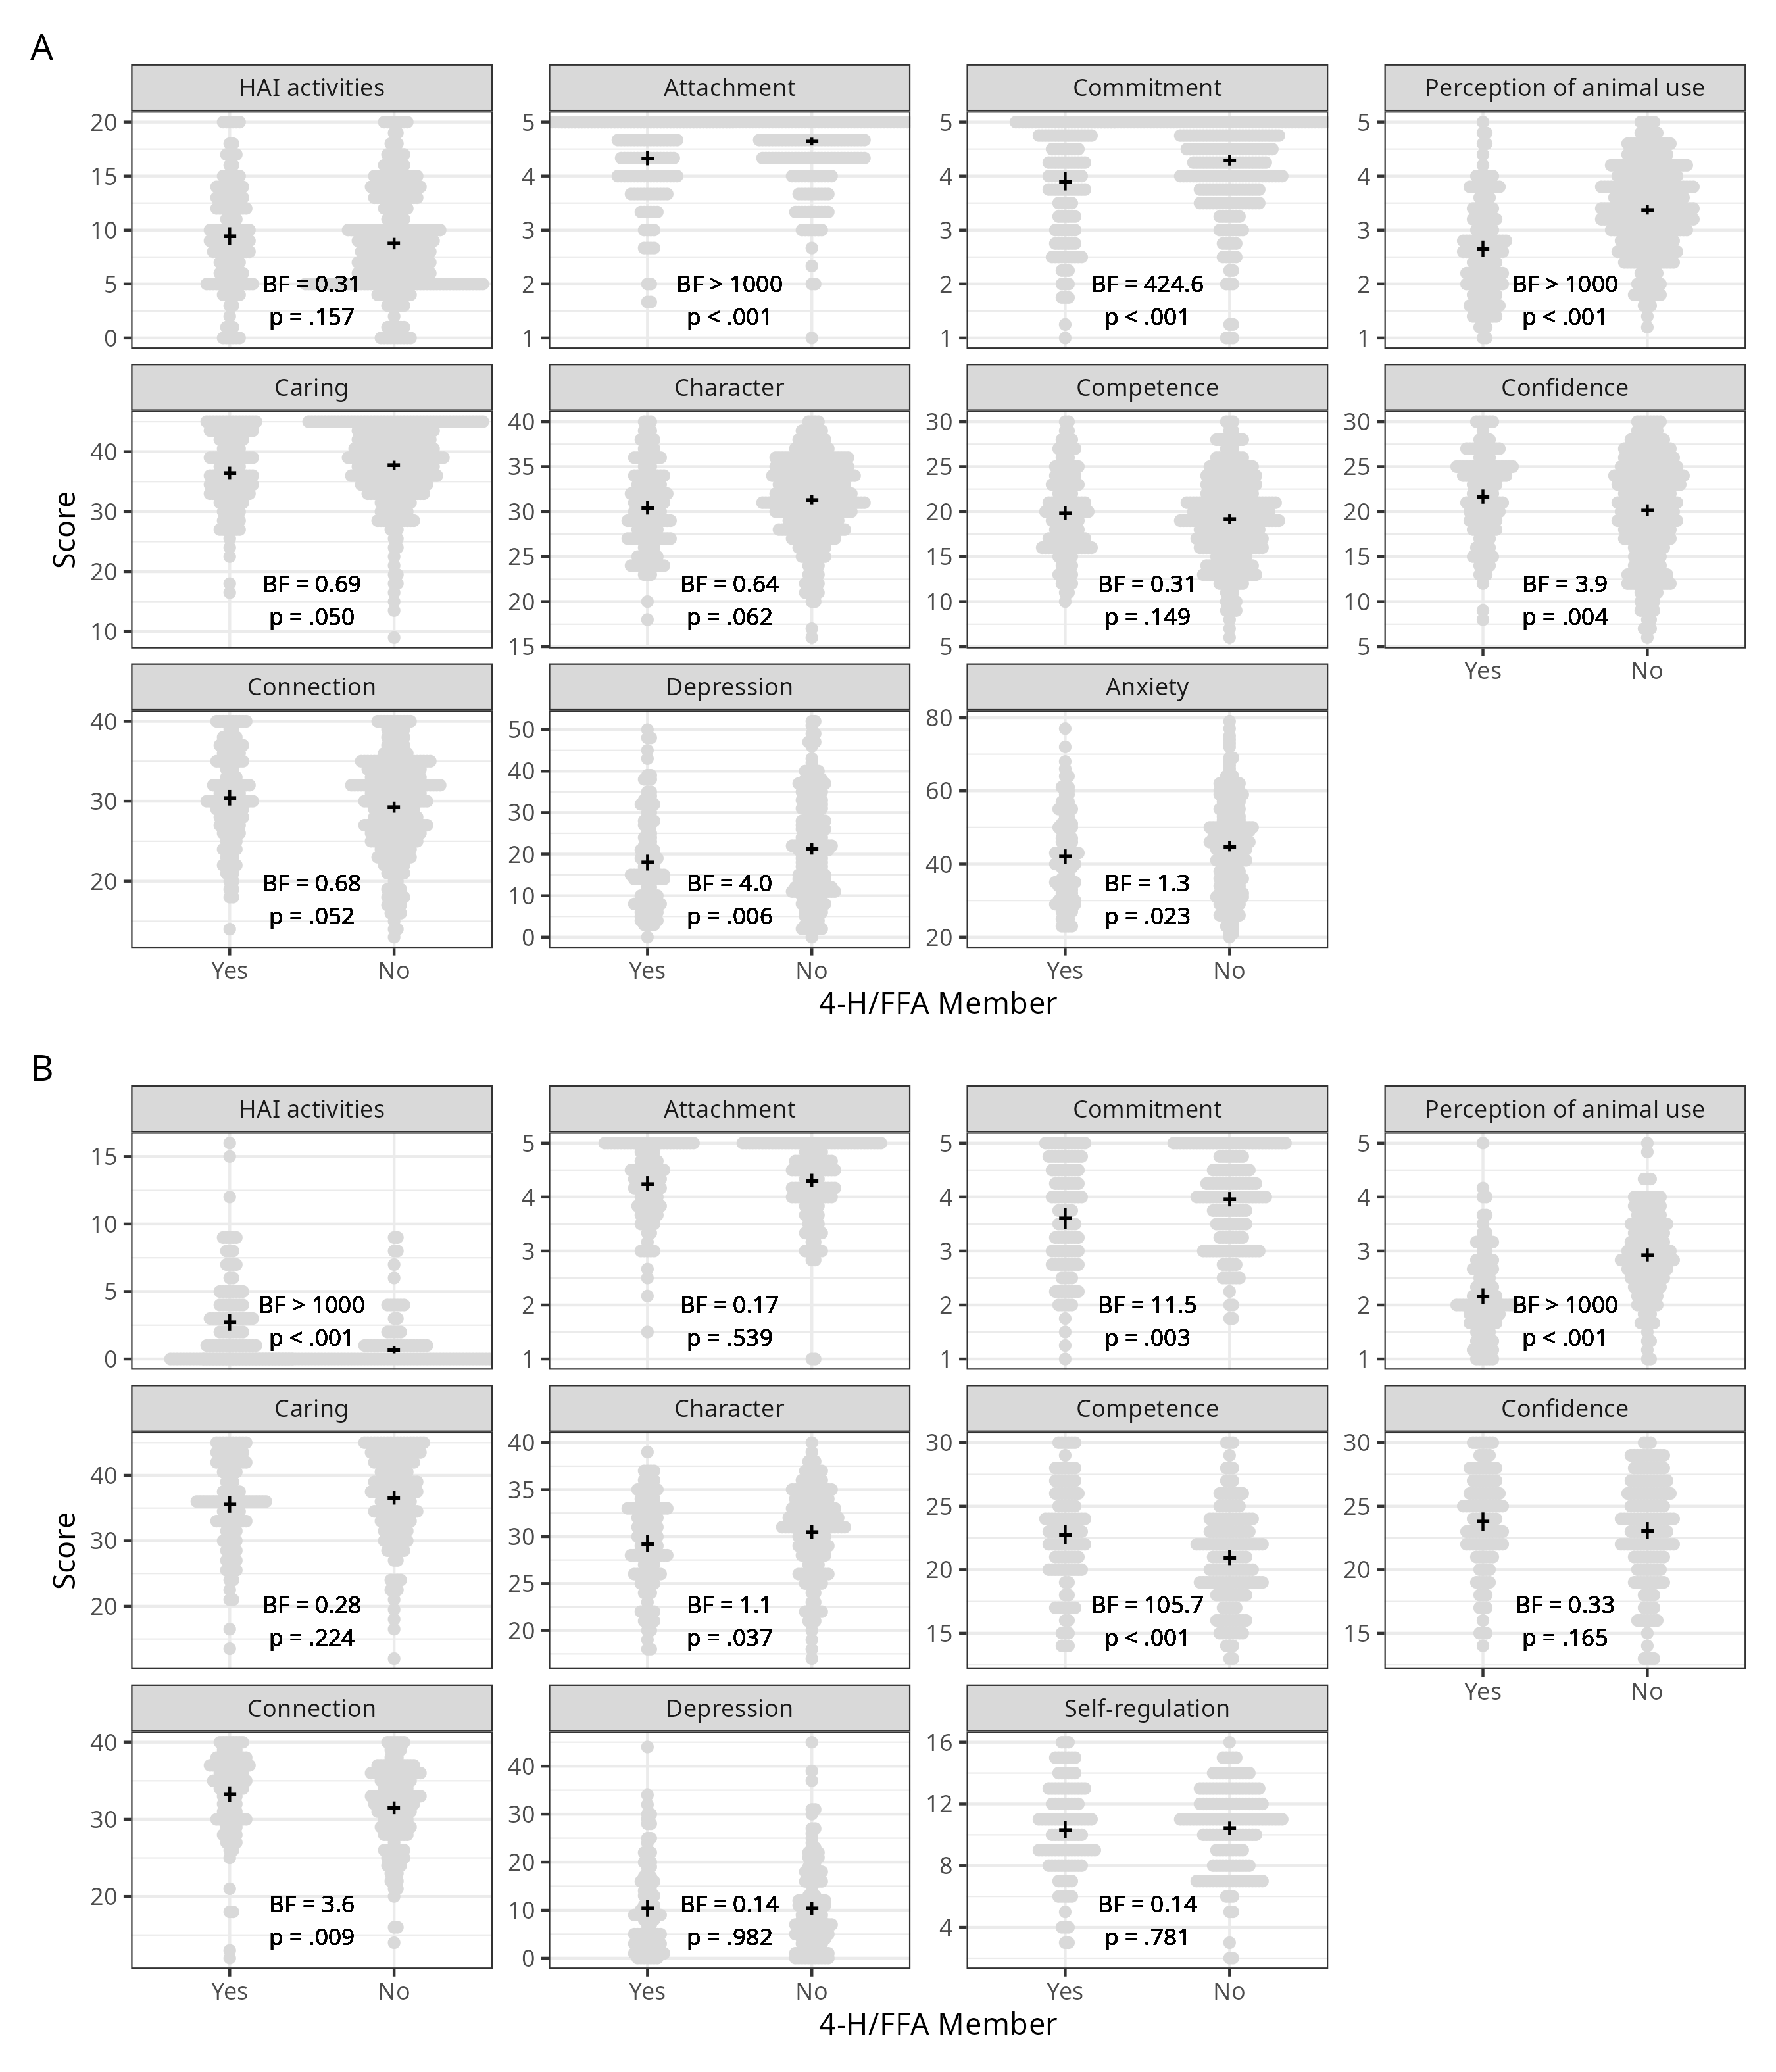
\includegraphics[width=9in,height=\textheight,keepaspectratio]{figures/group_diff_measures.png}

{\noindent \emph{Note.} Grey dots represent individual subject data
points, black horizontal bars represent group means, and black vertical
bars represent 95\% confidence intervals. Figure used with permission
under a CC-BY 4.0 license: Pachunka et al.~(2024); available at
https://doi.org/10.31234/osf.io/ge7bf.}

\end{figure}

To test for effects of group membership on the relationship between
human-animal interaction and positive youth development, we reran each
of the previously described structural equation models but included
membership as a moderator using a multigroup confirmatory factor
analysis. There was no evidence of moderation effects of membership into
4-H/FFA for these associations.

\section{Discussion}\label{discussion}

Our primary aim for these studies was to replicate and extend Mueller's
(\citeproc{ref-Mueller.2014}{2014}) findings about the relationship
between positive youth development and both human-animal interaction and
attitudes about animals. Mueller found that the positive youth
development component of contribution was positively associated with
animal ownership, amount of caring for animals, and the presence and
frequency of animal-related activities. Across our two studies, we did
not find an association with any human-animal interaction variables and
contribution. Instead, we found positive associations between animal
ownership and competence and confidence, amount of caring for an animal
and competence and self-regulation, and frequency of animal activities
and caring and depression. However, none of these associations were
found in both replicates of our studies---each only occurred in one
replicate. Thus, we failed to replicate Mueller's associations between
positive youth development and human-animal interaction, with minimal
replication of significant associations across our two studies.

Mueller (\citeproc{ref-Mueller.2014}{2014}) found a number of different
associations between positive youth development and measures of animal
attitudes (animal attachment, commitment, and perception of animal use).
Our Study 1 replicated 6 of the 12 associations found by Mueller. In
addition, we found another four associations not found by Mueller. In
Study 2, we only replicated 4 of Mueller's 12 associations and found an
additional four associations not found by Mueller. In all cases of
replication, the sign of the association was the same in both studies.
Thus, we partially replicated Mueller's associations between positive
youth development and animal attitudes. In terms of our internal
replication, 18 out of 21 of the association outcomes replicated between
our two studies.

Finally, we extended Mueller's (\citeproc{ref-Mueller.2014}{2014}) study
by comparing members of 4-H/FFA to non-members to investigate whether
this membership moderated any of the effects that we observed. Despite
some differences in human-animal interaction and positive youth
development characteristics between members and non-members, the
addition of membership as a moderator did not affect the models. Thus,
membership in 4-H/FFA did not influence the associations between
positive youth development and human-animal interaction or animal
attitudes.

\subsection{Implications}\label{implications}

\subsubsection{Human-Animal Interaction and Positive Youth
Development}\label{human-animal-interaction-and-positive-youth-development}

Our study examined the associations between positive youth development
and human-animal interaction across two studies, replicating and
extending Mueller's (\citeproc{ref-Mueller.2014}{2014}) methods. None of
our studies nor Mueller's original work demonstrated strong or
consistent effects of human-animal interaction on positive youth
development (Table~\ref{tbl-haieffects}). These findings suggest that
while human-animal interaction is often viewed as beneficial for youth
development, the evidence for direct associations between interacting
with animals and positive youth development outcomes is weak or highly
context dependent. While the literature on human-animal interaction
often highlights the emotional, social, and psychological benefits of
interacting with animals (\citeproc{ref-Beetz.etal.2011}{Beetz et al.,
2011}; \citeproc{ref-Melson.2003}{Melson, 2003}), our findings suggest
that these effects are not universal.

The inconsistency in effects across studies may reflect the complexity
of human-animal relationships. For instance, different types of
interactions (e.g., caregiving, companionship, competitive activities)
likely contribute differently to positive youth development. Companion
animals, for example, may foster empathy and responsibility in youth
(\citeproc{ref-Daly.Morton.2006}{Daly \& Morton, 2006}), while
competitive or labor-based interactions might not provide the same
nurturing environment. This nuance aligns with Overton's
(\citeproc{ref-Overton.2010}{2010}) relational developmental systems
theory, which emphasizes that positive youth development outcomes are
shaped by the reciprocal interaction between individuals and their
environments. In the case of human-animal interaction, the context in
which youth engage with animals, whether in structured programs like 4-H
and FFA or informal pet ownership, might dictate the developmental
benefits they receive. Thus, the lack of strong, consistent effects of
human-animal interaction on positive youth development across our
studies likely stems from the variability in how and why young people
interact with animals.

\subsubsection{Animal Attitudes and Positive Youth
Development}\label{animal-attitudes-and-positive-youth-development-1}

In contrast to the weak and inconsistent effects of human-animal
interaction on positive youth development, our studies found stronger
and more consistent associations between attitudes toward animals, such
as attachment, commitment, and perception of animal use, and positive
youth development outcomes (Table~\ref{tbl-cogeffects}). These results
suggest that the way young people think and feel about animals, rather
than simply their level of interaction, has a stronger association with
their developmental outcomes. One possible explanation is that attitudes
reflect deeper, internalized values that guide behavior, whereas
interactions may not have the same lasting impact unless they are tied
to emotional significance. Youths who exhibit high attachment or
commitment to animals may share traits like empathy, responsibility, and
care. Emotional bonds that youth form with animals may connect to traits
that align with positive youth development's core elements (e.g.,
caring, connection).

The stronger associations between animal attitudes and positive youth
development align with existing research on the role of emotions and
attitudes in youth development. For example, attachment to companion
animals contributes to children's emotional security and self-esteem
(\citeproc{ref-Zasloff.1996}{Zasloff, 1996}) and fosters empathy,
responsibility, and prosocial behaviors
(\citeproc{ref-Daly.Morton.2006}{Daly \& Morton, 2006};
\citeproc{ref-Melson.2003}{Melson, 2003}). In this context, youths'
emotional attachments to animals may serve as a pathway through which
they develop empathy and caring, essential components of positive youth
development. Thus, it is not just the presence of animals in youths'
lives that matters, but how they cognitively and emotionally engage with
those animals.

Perception of animal use emerged as one of the most consistent
predictors of positive youth development outcomes, particularly caring
and depression (Table~\ref{tbl-cogeffects}). This finding suggests that
young people's ethical beliefs about animal use (food production,
scientific research, etc.) are closely tied to their personal
development. Young people with lower acceptance of a variety of animal
uses likely demonstrate greater empathy and concern for others, a core
component of positive youth development's caring dimension
(\citeproc{ref-Mueller.2014}{Mueller, 2014}). The literature supports
this link, showing that individuals who advocate for animal welfare
often extend their empathy to human social causes as well, engaging in
prosocial activities and promoting justice
(\citeproc{ref-Herzog.etal.2015}{Herzog et al., 2015}).

Overall, our findings suggest that while human-animal interaction may
offer some developmental benefits, it is young people's emotional and
cognitive engagement with animals, particularly their attachment and
perception of animal use, that plays a more critical role in shaping
positive youth development outcomes. Programs aiming to leverage
human-animal interaction for youth development, such as 4-H and FFA,
should consider how a youth's emotional investment in their relationship
with animals may enhance positive youth development more effectively
than increasing the frequency or intensity of animal interactions.

\subsubsection{Group Membership}\label{group-membership-1}

One of the striking findings of this study is the lack of a difference
between youth involved with 4-H and FFA (members) and those not involved
(non-members) in terms of positive youth development. None of the Six Cs
differed between members and non-members consistently across both data
sets.

Though membership in 4-H and FFA have inconsistent relationships with
positive youth development, it shows more consistent relationships with
animal attitudes. Across both studies, non-members had higher commitment
and perception of animal use scores and in Study 1 non-members also had
higher attachment scores.

This study indicates that youth not affiliated with 4-H and FFA have
higher attachment and commitment to animals than those involved with 4-H
and FFA. However, non-members likely focused their interactions with
family pets, whereas members likely focused on livestock. In our Study
1, we found that 97.6\% of non-members choose pets over livestock,
whereas only 63.8\% of members chose pets. Thus, the two groups likely
had in mind different types of animals when completing our survey.

Our results also indicated that non-members had lower acceptance of
animal uses than members. Urban youth with less exposure to some animals
uses may be more likely to be less accepting of these practices. In
contrast, rural youth who interact daily with food animals (beef cattle,
dairy cattle, pigs, and sheep) would likely agree with the need for
humane treatment and respect of animals but be more willing to accept a
wider variety of animal uses.

We found several differences in human-animal interaction and positive
youth development characteristics between members and non-members.
However, 4-H/FFA membership did not influence associations between
positive youth development and human-animal interaction or animal
attitudes. While key differences exist between members and non-members
regarding background and context in development of key responses,
ultimately any repeated interaction with animals appears to provide
positive youth development, regardless of animal type and/or
facilitation of those activities.

\subsubsection{Failure to Replicate}\label{failure-to-replicate}

We partially replicated Mueller's (\citeproc{ref-Mueller.2014}{2014})
results, but we did not replicate several findings. We did not find an
association between human-animal interaction variables and contribution.
Additionally, the significant associations between other positive youth
development variables and human-animal interaction variables were not
consistent across our two studies. Overall, we observed smaller effect
sizes for the association between positive youth development and
human-animal interaction than those by Mueller. Our sample was slightly
smaller than Mueller's but had similar demographic characteristics.

We partially replicated Mueller's (\citeproc{ref-Mueller.2014}{2014})
associations between positive youth development and measures of animal
attitudes, replicating 6 out of the 12 significant associations reported
by Mueller. The larger effect sizes and greater consistency over our two
studies suggest that associations between positive youth development and
animal attitudes may be more strongly related than relationships between
positive youth development and human-animal interaction. We do not
conclude that there is no relationship between human-animal interaction
and positive youth development based on our results, but that the nature
of this relationship may be more complex and require larger sample sizes
to account for other sources of variance.

\subsection{Limitations and Future
Directions}\label{limitations-and-future-directions}

Our studies had several limitations. The measurement of human-animal
interaction is complex and may require additional study to describe the
quality and quantity of these interactions more accurately. It is also
possible that multiple other factors can also influence measures of
human-animal interaction in different ways. Future studies could refine
and validate measures of human-animal interaction, since there has been
a rapid proliferation of the number of possible scales
(\citeproc{ref-Samet.etal.2023}{Samet et al., 2023}).

Secondly, interpreting nonsignificant results in replication studies
(even in seemingly well-powered studies) is difficult for myriad reasons
and may necessitate multiple replication studies to provide firm
evidence for a hypothesis (\citeproc{ref-Maxwell.etal.2015}{Maxwell et
al., 2015}). These points all support further research focused on the
effects of human-animal interaction and animal attitudes on positive
youth development to help maximize youth development opportunities.

\subsection{Conclusion}\label{conclusion}

We replicated and extended the methods of Mueller
(\citeproc{ref-Mueller.2014}{2014}) to investigate the relationship
among human-animal interaction, animal attitudes, and positive youth
development. We did not find strong relationships among human-animal
interaction and positive youth development, which failed to replicate
Mueller's findings. However, we did find clear relationships between
animal attitudes and positive youth development, and many of these
effects replicated Mueller's findings. We extended Mueller's work by
considering membership in 4-H and/or FFA as a moderator in the analysis.
Though we found a few differences between members and non-members in
animal attitudes and positive youth development, these differences did
not moderate any relationships that we tested. Thus, we partially
replicated Mueller's original study, demonstrating that the relationship
between positive youth development and human-animal interactions and
animal attitudes is complex. The relationship between perception of
animal use and positive youth development seems to be fairly robust.
However, other animal attitudes and aspects of human-animal interaction
do not seem to have reliable relationships with positive youth
development. Future work in this area should ensure large sample sizes,
use strong measures of human-animal interaction and animal attitudes,
and consider the demographic and animal-relevant differences among
participants to better understand how animal relationships and attitudes
are related to positive youth development.

\section{Summary for Practitioners}\label{summary-for-practitioners}

Both interacting with animals and youth development programs, such as
4-H and FFA, have positively impacted participating youths' development
through improvement in skills such as accepting responsibility and
prosocial behavior (\citeproc{ref-Melson.2003}{Melson, 2003}). Little
research exists that investigates the benefits of human-animal
interaction in an individual's long-term development outside of
animal-assisted interventions and their immediate benefits. This study
applies to educators looking to incorporate animals into their youth
development programs. Our study surveyed university undergraduates about
their human-animal interactions (ownership, care, activities), animal
attitudes (animal attachment, commitment, and perception of animal use),
positive youth development outcomes (competence, connection, confidence,
character, and caring, contribution), and youth development activities
membership (4-H, FFA). We found that, although animal interactions or
membership in program did not have a strong correlation with positive
youth development outcomes, an individual's attitudes about animals did
correlate with positive youth development outcomes. However, the
benefits of interacting with animals as a method of impacting youth
development depend on the context.

Our work suggests that practitioners should focus on nourishing youth's
attitudes surrounding animals as they build their programs or curricula.
If a program's budget cannot afford to have their own animals, they can
still provide beneficial activities to youth that improve attitudes
towards animals. For example, our study found that individuals that
reported a higher attachment score also reported higher caring and
connection scores in positive youth development measures. Therefore, an
individual's attitudes towards animals is more strongly related to
developmental outcomes than whether they own or interact with an animal.
The depth of their emotional and cognitive engagement with animals is
more relevant in shaping their long-term development. Lastly, it is
crucial to be aware of the types of animals that individuals have
experience with to understand these context-dependent outcomes of
human-animal interaction. Our study found that members of 4-H and FFA
did not view their animals as pets or members of the family compared to
non-members. This is an important distinction as the type of animal an
individual has exposure to affects their attitudes towards animals.

\section{References}\label{references}

\phantomsection\label{refs}
\begin{CSLReferences}{1}{0}
\bibitem[\citeproctext]{ref-R-quarto}
Allaire, J., \& Dervieux, C. (2024). \emph{Quarto: R interface to
{``{Quarto}''} markdown publishing system}.
\url{https://github.com/quarto-dev/quarto-r}

\bibitem[\citeproctext]{ref-Baltes.etal.1999}
Baltes, P. B., Baltes, M. M., Freund, A. M., \& Lang, F. (1999).
\emph{The measurement of selection, optimization, and compensation
({SOC}) by self report: Technical report 1999}. Max-Planck-Institut
f{ü}r Bildungsforschung.

\bibitem[\citeproctext]{ref-Beetz.etal.2011}
Beetz, A., Kotrschal, K., Turner, D. C., Hediger, K., Uvnäs-Moberg, K.,
\& Julius, H. (2011). The effect of a real dog, toy dog and friendly
person on insecurely attached children during a stressful task: An
exploratory study. \emph{Anthrozo{ö}s}, \emph{24}(4), 349--368.
\url{https://doi.org/10.2752/175303711X13159027359746}

\bibitem[\citeproctext]{ref-Benson.etal.1998}
Benson, P. L., Leffert, N., Scales, P. C., \& Blyth, D. A. (1998).
Beyond the 'village' rhetoric: Creating healthy communities for children
and adolescents. \emph{Applied Developmental Science}, \emph{2}(3),
138--159. \url{https://doi.org/10.1207/s1532480xads0203_3}

\bibitem[\citeproctext]{ref-Bentler.1990}
Bentler, P. M. (1990). Comparative fit indexes in structural models.
\emph{Psychological Bulletin}, \emph{107}(2), 238--246.
\url{https://doi.org/10.1037/0033-2909.107.2.238}

\bibitem[\citeproctext]{ref-Bowers.etal.2010}
Bowers, E. P., Li, Y., Kiely, M. K., Brittian, A., Lerner, J. V., \&
Lerner, R. M. (2010). The {Five Cs} model of positive youth development:
A longitudinal analysis of confirmatory factor structure and measurement
invariance. \emph{Journal of Youth and Adolescence}, \emph{39}(7),
720--735. \url{https://doi.org/10.1007/s10964-010-9530-9}

\bibitem[\citeproctext]{ref-Daly.Morton.2006}
Daly, B., \& Morton, L. L. (2006). An investigation of human-animal
interactions and empathy as related to pet preference, ownership,
attachment, and attitudes in children. \emph{Anthrozo{ö}s},
\emph{19}(2), 113--127. \url{https://doi.org/10.2752/089279306785593801}

\bibitem[\citeproctext]{ref-Damon.2004}
Damon, W. (2004). What is positive youth development? \emph{The ANNALS
of the American Academy of Political and Social Science}, \emph{591}(1),
13--24. \url{https://doi.org/10.1177/0002716203260092}

\bibitem[\citeproctext]{ref-Davis.1980}
Davis, M. H. (1980). A multidimensional approach to individual
differences in empathy. \emph{JSAS Catalog of Selected Documents in
Psychology}, \emph{10}(4), 1--17.

\bibitem[\citeproctext]{ref-Eisenberg.etal.1996}
Eisenberg, N., Fabes, R. A., Murphy, B., Karbon, M., Smith, M., \&
Maszk, P. (1996). The relations of children's dispositional
empathy-related responding to their emotionality, regulation, and social
functioning. \emph{Developmental Psychology}, \emph{32}(2), 195--209.
\url{https://doi.org/10.1037/0012-1649.32.2.195}

\bibitem[\citeproctext]{ref-Geldhof.etal.2014}
Geldhof, G. J., Bowers, E. P., Boyd, M. J., Mueller, M. K., Napolitano,
C. M., Schmid, K. L., Lerner, J. V., \& Lerner, R. M. (2014). Creation
of short and very short measures of the five {Cs} of positive youth
development. \emph{Journal of Research on Adolescence}, \emph{24}(1),
163--176. \url{https://doi.org/10.1111/jora.12039}

\bibitem[\citeproctext]{ref-Harter.1988}
Harter, S. (1988). \emph{Manual for the {Self-perception Profile} for
{Adolescents}}. University of Denver.

\bibitem[\citeproctext]{ref-Herzog.etal.2015}
Herzog, H., Grayson, S., \& McCord, D. (2015). Brief measures of the
{Animal Attitude Scale}. \emph{Anthrozo{ö}s}, \emph{28}(1), 145--152.
\url{https://doi.org/10.2752/089279315X14129350721894}

\bibitem[\citeproctext]{ref-Hu.Bentler.1999}
Hu, L., \& Bentler, P. M. (1999). Cutoff criteria for fit indexes in
covariance structure analysis: {Conventional} criteria versus new
alternatives. \emph{Structural Equation Modeling}, \emph{6}(1), 1--55.
\url{https://doi.org/10.1080/10705519909540118}

\bibitem[\citeproctext]{ref-Jelicic.etal.2007}
Jelicic, H., Bobek, D. L., Phelps, E., Lerner, R. M., \& Lerner, J. V.
(2007). Using positive youth development to predict contribution and
risk behaviors in early adolescence: {Findings} from the first two waves
of the 4-{H Study} of {Positive Youth Development}. \emph{International
Journal of Behavioral Development}, \emph{31}(3), 263--273.
\url{https://doi.org/10.1177/0165025407076439}

\bibitem[\citeproctext]{ref-Johnson.etal.1992}
Johnson, T. P., Garrity, T. F., \& Stallones, L. (1992). Psychometric
evaluation of the {Lexington Attachment} to {Pets Scale} ({LAPS}).
\emph{Anthrozo{ö}s}, \emph{5}(3), 160--175.
\url{https://doi.org/10.2752/089279392787011395}

\bibitem[\citeproctext]{ref-Joreskog.1971}
Jöreskog, K. G. (1971). Simultaneous factor analysis in several
populations. \emph{Psychometrika}, \emph{36}(4), 409--426.
\url{https://doi.org/10.1007/BF02291366}

\bibitem[\citeproctext]{ref-Lerner.etal.2005}
Lerner, R. M., Lerner, J. V., Almerigi, J. B., Theokas, C., Phelps, E.,
Gestsdottir, S., Naudeau, S., Jelicic, H., Alberts, A., Ma, L., Smith,
L. M., Bobek, D. L., Richman-Raphael, D., Simpson, I., Christiansen, E.
D., \& Von Eye, A. (2005a). Positive youth development, participation in
community youth development programs, and community contributions of
fifth-grade adolescents: Findings from the first wave of the 4-{H} study
of positive youth development. \emph{The Journal of Early Adolescence},
\emph{25}(1), 17--71. \url{https://doi.org/10.1177/0272431604272461}

\bibitem[\citeproctext]{ref-Lerner.etal.2005a}
Lerner, R. M., Wertlieb, D., \& Jacobs, F. (2005b). Historical and
theoretical bases of applied developmental science. In R. M. Lerner, D.
Wertlieb, \& F. Jacobs (Eds.), \emph{Applied {Developmental Science}:
{An Advanced Textbook}} (Vol. 1). SAGE.
\url{https://doi.org/10.4135/9781452233512.n1}

\bibitem[\citeproctext]{ref-MacCallum.etal.1996}
MacCallum, R. C., Browne, M. W., \& Sugawara, H. M. (1996). Power
analysis and determination of sample size for covariance structure
modeling. \emph{Psychological Methods}, \emph{1}(2), 130--149.
\url{https://doi.org/10.1037/1082-989X.1.2.130}

\bibitem[\citeproctext]{ref-Maxwell.etal.2015}
Maxwell, S. E., Lau, M. Y., \& Howard, G. S. (2015). Is psychology
suffering from a replication crisis? {What} does {``failure to
replicate''} really mean? \emph{American Psychologist}, \emph{70}(6),
487--498. \url{https://doi.org/10.1037/a0039400}

\bibitem[\citeproctext]{ref-Melson.2003}
Melson, G. F. (2003). Child development and the human-companion animal
bond. \emph{American Behavioral Scientist}, \emph{47}(1), 31--39.
\url{https://doi.org/10.1177/0002764203255210}

\bibitem[\citeproctext]{ref-R-BayesFactor}
Morey, R. D., \& Rouder, J. N. (2024). \emph{BayesFactor: Computation of
{Bayes} factors for common designs}.
\url{https://richarddmorey.github.io/BayesFactor/}

\bibitem[\citeproctext]{ref-Mueller.2014}
Mueller, M. K. (2014). Is human-animal interaction ({HAI}) linked to
positive youth development? {Initial} answers. \emph{Applied
Developmental Science}, \emph{18}(1), 5--16.
\url{https://doi.org/10.1080/10888691.2014.864205}

\bibitem[\citeproctext]{ref-OHaire.2010}
O'Haire, M. (2010). Companion animals and human health: {Benefits},
challenges, and the road ahead. \emph{Journal of Veterinary Behavior},
\emph{5}(5), 226--234. \url{https://doi.org/10.1016/j.jveb.2010.02.002}

\bibitem[\citeproctext]{ref-Overton.2010}
Overton, W. F. (2010). Life-span development: Concepts and issues. In R.
M. Lerner, M. E. Lamb, \& A. M. Freund (Eds.), \emph{The {Handbook} of
{Life}-{Span Development}} (1st ed.). Wiley.
\url{https://doi.org/10.1002/9780470880166.hlsd001001}

\bibitem[\citeproctext]{ref-Pachunka.etal.2024}
Pachunka, A., Jeffries, J., Karr, L., Luck, L., Reiling, B., Schultz,
D., \& Stevens, J. R. (2024). \emph{Effects of human-animal interaction
on positive youth development: {A} replication study}. PsyArXiv.
\url{https://doi.org/10.31234/osf.io/ge7bf}

\bibitem[\citeproctext]{ref-Phelps.etal.2009}
Phelps, E., Zimmerman, S., Warren, A. E. A., Jeličić, H., von Eye, A.,
\& Lerner, R. M. (2009). The structure and developmental course of
{Positive Youth Development} ({PYD}) in early adolescence:
{Implications} for theory and practice. \emph{Journal of Applied
Developmental Psychology}, \emph{30}(5), 571--584.
\url{https://doi.org/10.1016/j.appdev.2009.06.003}

\bibitem[\citeproctext]{ref-Piper.Uttley.2019}
Piper, L. J., \& Uttley, C. M. (2019). Adolescents and pets. In
\emph{Clinician's {Guide} to {Treating Companion Animal Issues}} (pp.
47--75). Elsevier.
\url{https://doi.org/10.1016/B978-0-12-812962-3.00004-6}

\bibitem[\citeproctext]{ref-R-base}
R Core Team. (2025). \emph{R: A language and environment for statistical
computing}. R Foundation for Statistical Computing.
\url{https://www.R-project.org/}

\bibitem[\citeproctext]{ref-Radloff.1977}
Radloff, L. S. (1977). The {CES-D} scale: A self-report depression scale
for research in the general population. \emph{Applied Psychological
Measurement}, \emph{1}(3), 385--401.
\url{https://doi.org/10.1177/014662167700100306}

\bibitem[\citeproctext]{ref-R-lavaan}
Rosseel, Y. (2012). {lavaan}: An {R} package for structural equation
modeling. \emph{Journal of Statistical Software}, \emph{48}(2), 1--36.
\url{https://doi.org/10.18637/jss.v048.i02}

\bibitem[\citeproctext]{ref-Samet.etal.2023}
Samet, L., Vaterlaws-Whiteside, H., Upjohn, M., \& Casey, R. (2023).
Status of instrument development in the field of human-animal
interactions \& bonds: {Ten} years on. \emph{Society \& Animals},
\emph{32}(1), 74--94. \url{https://doi.org/10.1163/15685306-bja10123}

\bibitem[\citeproctext]{ref-R-apaquarto}
Schneider, W. J. (2024). \emph{{apaquarto}}.
\url{https://wjschne.github.io/apaquarto}

\bibitem[\citeproctext]{ref-Small.Rodgers.1995}
Small, S., \& Rodgers, K. B. (1995). Teen {Assessment Project} ({TAP})
survey question bank. \emph{Madison: University of Wisconsin-Madison}.

\bibitem[\citeproctext]{ref-Spielberger.1983}
Spielberger, C. D. (1983). \emph{State-trait anxiety inventory for
adults}. American Psychological Association.
\url{https://doi.org/10.1037/t06496-000}

\bibitem[\citeproctext]{ref-Staats.etal.1996}
Staats, S., Miller, D., Carnot, M. J., Rada, K., \& Turnes, J. (1996).
The {Miller-Rada Commitment} to {Pets Scale}. \emph{Anthrozo{ö}s},
\emph{9}(2-3), 88--94. \url{https://doi.org/10.2752/089279396787001509}

\bibitem[\citeproctext]{ref-Yuan.Bentler.2000}
Yuan, K.-H., \& Bentler, P. M. (2000). Three likelihood-based methods
for mean and covariance structure analysis with nonnormal missing data.
\emph{Sociological Methodology}, \emph{30}(1), 165--200.
\url{https://doi.org/10.1111/0081-1750.00078}

\bibitem[\citeproctext]{ref-Zasloff.1996}
Zasloff, R. L. (1996). Measuring attachment to companion animals: A dog
is not a cat is not a bird. \emph{Applied Animal Behaviour Science},
\emph{47}(1-2), 43--48.
\url{https://doi.org/10.1016/0168-1591(95)01009-2}

\end{CSLReferences}






\end{document}
